\documentclass{dcthesis}

\usepackage{graphicx}
\usepackage{setspace}
\usepackage{amssymb,amsthm,amsmath,amstext}
\usepackage{mathrsfs}  % allows nice script font for sheaves
% \usepackage{bm}        % allows bold italic letters in math mode
% \usepackage{mathtools} % allows more extendible arrows
\usepackage{stmaryrd}  % additional nice fonts
\usepackage{mathtools}
\usepackage{geometry}
\usepackage{xy}
\usepackage{algorithm}
\usepackage{algpseudocode}
\usepackage{lipsum}
\usepackage{caption}
\usepackage{tikz-cd}
\usepackage{bbm}
\usepackage{hyperref}
\hypersetup{
    colorlinks=true,
    linkcolor=blue,
    filecolor=magenta,      
    urlcolor=cyan,
    pdftitle={Overleaf Example},
    pdfpagemode=FullScreen,
    }


\DeclareCaptionFormat{algor}{%
  \hrulefill\par\offinterlineskip\vskip1pt%
    \textbf{#1#2}#3\offinterlineskip\hrulefill}
\DeclareCaptionStyle{algori}{singlelinecheck=off,format=algor,labelsep=space}
\captionsetup[algorithm]{style=algori}

%This version of the thesis template has been updated for the February 2017 thesis guidelines provided by the School of Graduate and Advanced Studies by David Freund and Daryl DeFord.

%  Some good options are draft and singlespacing, for drafts, and *final*,
%for the final cut, and noheadings, for a printout without headings.  
%You can also use the copyright option to add a copyright.  Note:
%final will enforce a bunch of different options, like oneside, 12pt
%and doublespacing, as well as make the margins correct.   Draft, has
%larger margins and is appropriate for twosided printing.   


%%%%%%%%%%%%%%%%%%%%%%%%%%%
%%%%    IMPORTANT     %%%%%
%%%%%%%%%%%%%%%%%%%%%%%%%%%
%
%  Because dvips doesn't know/care about the page size of the dvi file
%  its working on, and because its so important that the margins of
%  your thesis are correct you have to make sure that you are using
%  the command dvi -t letter *thesisnamehere*
%
%  If you are using a terminal this is straightforward, but if you are
%  using a tex editing program it make take a little bit of searching
%  before you figure out how to make this work. 
%  
%  Alternatively, you might consider compiling using pdflatex, which
%  compiles straight to a PDF and doesn't have this problem.  

%%%%%%%%%%%%%%%%%%%%%%%%%%%%%%%%%%%%%%%%%%%%%%%%%%
% Additional Packages (add as desired)
%%%%%%%%%%%%%%%%%%%%%%%%%%%%%%%%%%%%%%%%%%%%%%%%%%
\usepackage{amsmath,amssymb,amsthm}

%\usepackage{mkindex} %Uncomment if you would like to have an index. Compiling with an index takes more work than compiling without one. You will have to look up how to use the index package.

%%%%%%%%%%%%%%%%%%%%%%%%%%%%%%%%%%%%%%%%%%%%%%%%%%
%Formatting
%%%%%%%%%%%%%%%%%%%%%%%%%%%%%%%%%%%%%%%%%%%%%%%%%%
%  Change or add to as desired. 
%  These two commands make the first enumerations look like (a)
%  And the second level like (i).  
\renewcommand{\labelenumi}{(\alph{enumi})}
\renewcommand{\labelenumii}{(\roman{enumii})}
%  These commands make the section headings Boldface and not all
%  caps. It also removes the chapter numbers  
\renewcommand{\chaptermark}[1]{\markboth{{\sc #1}}{{\sc #1}}}
\renewcommand{\sectionmark}[1]{\markright{{\sc \thesection\ #1}}}
%  These commands have lowercase headings with chapter numbers. 
%\renewcommand{\chaptermark}[1]{markboth{#1}{}}
%\renewcommand{\sectionmark}[1]{\markright{\thesection\ #1}} 
		
%%%%%%%%%%%%%%%%%%%%%%%%%%%%%%%%%%%%%%%%%%%%%%%%%%
% Theorem Declarations
%%%%%%%%%%%%%%%%%%%%%%%%%%%%%%%%%%%%%%%%%%%%%%%%%%
% A basic set of theorem declarations.  Add or remove as desired. 
\newtheorem{prop}{Proposition}[chapter]
\newtheorem{theorem}[prop]{Theorem}
\newtheorem{lemma}[prop]{Lemma}
\newtheorem{corr}[prop]{Corollary}
\theoremstyle{definition}
\newtheorem{definition}[prop]{Definition}
\theoremstyle{remark}
\newtheorem{remark}[prop]{Remark}
\newtheorem{example}[prop]{Example}
\newtheorem*{claim}{Claim}


%%%%%%%%%%%%%%%%%%%%%%%%%%%%%%%%%%%%%%%%%%%%%%%%%%
%Indicies
%%%%%%%%%%%%%%%%%%%%%%%%%%%%%%%%%%%%%%%%%%%%%%%%%%
%This is for an index.  More work is neede for a notation index
%\makeindex

%%%%%%%%%%%%%%%%%%%%%%%%%%%%%%%%%%%%%%%%%%%%%%%%%%
% Macros
%%%%%%%%%%%%%%%%%%%%%%%%%%%%%%%%%%%%%%%%%%%%%%%%%%
% Add your math macros here

%%%%%%%%%%%%%%%%%%%%%%%%%%%%%%%%%%%%%%%%%%%%%%%%%%
% Title Page Information
%%%%%%%%%%%%%%%%%%%%%%%%%%%%%%%%%%%%%%%%%%%%%%%%%%
%  Your personal info goes here!
\title{Cracking Enigma}
\subtitle{The Mathematics and Circuitry that Bested German Cryptographers}
\author{Jonah Weinbaum}

\begin{document}

%%%%%%%%%%%%%%%%%%%%%%%%%%%%%%%%%%%%%%%%%%%%%%%%%%
%Front end of thesis
%%%%%%%%%%%%%%%%%%%%%%%%%%%%%%%%%%%%%%%%%%%%%%%%%%
\frontmatter

\newgeometry{left=1.5in,top=1in,bottom=1in,right=1in}
\maketitle
\restoregeometry

%%%%%%%%%%%%%%%%%%%%%%%%%%%%%%%%%%%%%%%%%%%%%%%%%%
%Abstract
%%%%%%%%%%%%%%%%%%%%%%%%%%%%%%%%%%%%%%%%%%%%%%%%%%


%%%%%%%%%%%%%%%%%%%%%%%%%%%%%%%%%%%%%%%%%%%%%%%%%%
%Table of Contents
%%%%%%%%%%%%%%%%%%%%%%%%%%%%%%%%%%%%%%%%%%%%%%%%%%
\tableofcontents

%Add a list of tables
%\listoftables

%Add a list of figures
%\listoffigures

%%%%%%%%%%%%%%%%%%%%%%%%%%%%%%%%%%%%%%%%%%%%%%%%%%
%Main Portion of Thesis
%%%%%%%%%%%%%%%%%%%%%%%%%%%%%%%%%%%%%%%%%%%%%%%%%%
\mainmatter

%%%%%%%%%%%%%%%%%%%%%%%%%
%%  YOUR THESIS HERE!  %%
%%%%%%%%%%%%%%%%%%%%%%%%%

\chapter{The Enigma}

% \begin{chapquote}{Gordon Welchman, \textit{The Hut Six Story Page 52}}
%   The Enigma, though simple in principle and primitive in many ways,
%   presented the cryptanalyst with a dazzling number of possibilities.
% \end{chapquote}

The Enigma machine was used extensively by the Germans to encipher
communications prior to and throughout World War II. German
stratagems like the \emph{blitzkrieg} required quick radio
%% See the Code Book Singh page 196 %%
communication, so to ensure that the allied powers did not intercept
signals, they encoded all radio signals using the Enigma machine.
Breaking the Enigma would allow the allied powers to freely intercept
all naval, air force, and military command -- offering them time to
counter, defend, and retaliate appropriately. 
% Thus, while millions
% participated in a war of arms and power, a select group of academics
% at Bletchley Park engaged in a battle of minds to crack a puzzle
% whose solution could save millions of lives.

\section{The Machine}
Throughout this paper, the model \texttt{I} Enigma is chosen to
represent our canonical machine as these were the most common version
used during World War II with over 20000 being produced. Further, it
was used by both the \emph{Heer} (Army), \emph{Luftwaffe} (Air
Force), and the \emph{Kriegsmarine} (Navy), making this a prime target
for attack by cryptanalysts. Many models existed, each with varying
layouts, key spaces, and use-cases; however, the central ideas that
are discussed in this paper can generally be adapted to work on other models.
\\\\At its most basic function, the Enigma (once set up) is a
keyboard whose letters, when depressed, illuminate bulbs of a
corresponding keyboard layout. The operator presses keys of the
desired plain-text and copies the output of the illuminated bulbs to
obtain the enciphered text. The actual mechanism of this encipherment
requires several mechanical components in a complex arrangement.

\subsection{The Plugboard}

% \begin{figure}[htbp]
%   \begin{center}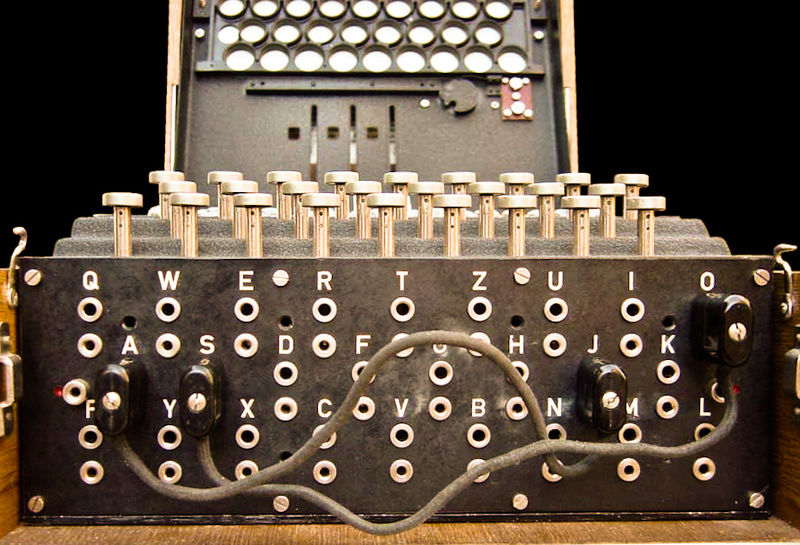
\includegraphics[scale=0.9]{images/plugboard.jpg}
%   \end{center}
%   \label{ref:plugboard}
%   \caption{Enigma \texttt{I} Plugboard}
% \end{figure}

Upon a key press, the electrical current corresponding to this letter
is sent to a mechanism known as the {\bf{plugboard}}. From an operator's
perspective, the plugboard was a series of ports, one for each
letter, along with 10 cables which could connect these ports. When
two letters are connected via a cable (e.g. A and Z), the plugboard
will send current corresponding to a letter to the opposite letter
(e.g. A goes to Z and vice versa). If no cable is plugged in to a
letter (e.g. D has no cable), then the plugboard simply will return a
current corresponding to this same letter (e.g. D). When a letter is connected to another 
through the plugboard, we will say that the letters are {\bf{steckered}} to one another. Assuming all 10
cables are used, this means that the plugboard can be represented as a
permutation on 26 letters with $2^{10}1^6$ cycle type\footnote{We
  will denote cycle types in this paper in the format
  $\lambda_1^{m_1}\dots\lambda_k^{m_k}$ where $\lambda_i$ is the length
of a cycle and $m_i$ is the multiplicity of this cycle length. We will often write the full notation $1^{m_1}\dots n^{m_n}$ in which $m_i$ may be $0$.}. One such
permutation could be
\begin{center}
  (\texttt{HR})(\texttt{AT})(\texttt{IW})(\texttt{SK})(\texttt{UY})(\texttt{DF})(\texttt{GV})(\texttt{LJ})(\texttt{BQ})(\texttt{MX})(\texttt{C})(\texttt{E})(\texttt{N})(\texttt{O})(\texttt{P})(\texttt{Z}).
\end{center}
In general, we will denote the permutation corresponding to a plugboard as $S$.

\subsection{The Rotors}
% \begin{figure}[htpb]
%   \centering
%   \begin{subfigure}{0.3\textwidth}
%     \includegraphics[width=\linewidth]{images/rotor_v_front.jpg}
%     \caption{Entry-side}
%     \label{fig:rotor_v_front}
%   \end{subfigure}
%   \hspace{0.02\textwidth}
%   \begin{subfigure}{0.3\textwidth}
%     \includegraphics[width=\linewidth]{images/rotor_v_back.jpg}
%     \caption{Exit-side}
%     \label{fig:rotor_v_back}
%   \end{subfigure}
%   \caption{Rotor \texttt{V}}
%   \label{fig:rotor_v}
% \end{figure}

The Enigma model \texttt{I} used three rotors, selected from a larger
set of rotors, the number of which changed depending on the military
branch we examine. At a minimum, all three branches of the military
had access to five rotors labeled by their roman numeral equivalents (i.e. $\texttt{I},\dots,\texttt{V}$).
Each rotor encoded a unique permutation from 26 input contacts to 26
output contacts by simply connecting between each input/output pair
in the permutation with a wire. The contacts represent the letters
in alphabetical order moving in a clockwise manner relative to the
entry side of the rotor. The input contacts of the rotor were often marked
with a white dot indicating which contact corresponded to \texttt{A},
but in general is found by looking at the contact immediately above
the numeral indicator.
\\\\On their own, these rotors would prove to be very poor
cryptographic devices, as they are just substitution ciphers, which are
vulnerable to frequency analysis and, if found by the enemy, would
serve no purpose whatsoever. Therefore, these rotors were designed to
rotate, which served to change the substitution at each stage of encryption.
\\\\Because these rotors rotate, it is best to differentiate between
contact letters and contact positions. When we give the permutation
corresponding to a rotor as in figure \ref{fig:rotor_v_wiring} we are
referring to the \texttt{A} contact as the specific contact denoted
by the marker dot and the \texttt{B} contact as its next contact
turning clockwise. When referred to in this context, we will use the
word ``contact''. On the other hand, when we say that an electrical
current corresponding to \texttt{A} enters a rotor, we mean
that the current enters the contact at the topmost \emph{position} of
the rotor, even if the rotor has rotated now so that that contact
is not the contact with the marker dot. When referred to in this
context we will use the word ``position'' so as to disambiguate from
the prior context. That is to say, a contact and a position need not
be the same. For example, contact \texttt{A} can be in position
\texttt{B}. This occurs when the pin with the marker dot adjacent to
it is one pin away from being at the top of the rotor.

\subsubsection{Turnover}
Each rotor had on its entry-side a notch next to each contact. A pawl
attempted to engage
the notch and move the rotor forward by one contact each key press.
On the exit-side, each
rotor was equipped with a smooth ring with only a single notch
breaking it. This is known as the {\bf{turnover notch}}. Assuming the
rotor functions in isolation the pawl will engage the entry notches
during each key press thus moving the rotor forward by one until,
after 26 presses, the rotor returns to its original position.
However, if we have two rotors, say rotor M and N, such that rotor M
has its entry contacts placed adjacent to the exit contacts of rotor
N; then, the smooth ring of the rotor N will occlude the notches of
rotor M thus preventing the pawl from engaging. That is, except at
the location where the turnover notch is located. The pawl will then
only be able to rotate rotor M if it aligns with the turnover notch of rotor N.
\\\\Now consider three rotors, rotors L, M, and N, arranged left to
right from an operator's perspective. Then electrical current first
enters rotor N, followed by rotor M, and finally rotor L. Rotor N
will have no rotor's smooth ring occluding its notches so the pawl is
free to engage rotor N at every key press. Thus rotor N will always
turn at each press of the key. Rotor M, however, will only turn at
the position at which rotor N's turnover notch aligns with the pawl
(save for a case we will shortly discuss),
meaning that for each full rotation of rotor N, rotor M will move
by one contact. Finally, rotor L will only move when rotor M's
turnover notch is aligned with the pawl, meaning that rotor N must make 26 full rotations before rotor L will move by one contact.

%% https://www.cryptomuseum.com/crypto/enigma/m3/index.htm %%
\begin{center}
  \begin{figure}[h]
    \[
      \left(
        \begin{array}{llllllllllllllllllllllllll}
          \texttt{A} & \texttt{B} & \texttt{C} & \texttt{D} &
          \texttt{E} & \texttt{F} & \texttt{G} & \texttt{H} &
          \texttt{I} & \texttt{J} & \texttt{K} & \texttt{L} &
          \texttt{M} & \texttt{N} & \texttt{O} & \texttt{P} &
          \texttt{Q} & \texttt{R} & \texttt{S} & \texttt{T} &
          \texttt{U} & \texttt{V} & \texttt{W} & \texttt{X} &
          \texttt{Y} & \texttt{Z}                             \\
          \texttt{V} & \texttt{Z} & \texttt{B} & \texttt{R} &
          \texttt{G} & \texttt{I} & \texttt{T} & \texttt{Y} &
          \texttt{U} & \texttt{P} & \texttt{S} & \texttt{D} &
          \texttt{N} & \texttt{H} & \texttt{L} & \texttt{X} &
          \texttt{A} & \texttt{W} & \texttt{M} & \texttt{J} &
          \texttt{Q} & \texttt{O} & \texttt{F} & \texttt{E} &
          \texttt{C} & \texttt{K}
        \end{array}
      \right)
    \]
    \caption{Rotor \texttt{V} permutation}
    \label{fig:rotor_v_wiring}
  \end{figure}
\end{center}

\subsubsection{Double Stepping}\label{double_step}
Arguably the most confusing aspect of the mechanics of the Enigma
machine is that of the {\bf{double step}}. We just said that the each
of the left two rotors ($M$ and $L$) can \emph{only} be moved when
the turnover notch of its right-hand adjacent rotor ($N$ and $M$
respectively) is aligned with the pawl. For $L$ this is true.
However, for rotor $M$, we must consider that even if rotor $N$'s
turnover notch is \emph{not} aligned with the pawl, rotor $M$'s own
turnover notch \emph{may} be aligned with the pawl. In this case, the
pawl will engage and move $L$; however, the turnover notch is still
connected to rotor $M$, so when the pawl engages $M$'s turnover notch
it will not only move $L$, but it will also move $M$ (just from the opposite side that we might expect).
\\\\We will illustrate this effect by example. Suppose our rotors
$N$, $M$, and $L$ had only three positions ($1$, $2$, and $3$). They
will each have a turnover notch aligned with a pawl when at position
$1$. We will walk through a full cycle of turnover of the leftmost
rotor $L$ step-by-step. We have
\begin{itemize}
  \item (Step $0$) $L = 2$, $M = 2$, $N = 3$ -- This represents our
    initial position
  \item (Step $1$) $L = 2$, $M = 2$, $N = 1$ -- Pawl engages $N$ and
    steps it forward
  \item (Step $2$) $L = 2$, $M = 3$, $N = 2$ -- Pawl engages $N$ and
    $N$'s turnover notch engages $M$.
  \item (Step $3$) $L = 2$, $M = 3$, $N = 3$ -- Pawl engages $N$ and
    steps it forward
  \item (Step $4$) $L = 2$, $M = 3$, $N = 1$ -- Pawl engages $N$ and
    steps it forward
  \item (Step $5$) $L = 2$, $M = 1$, $N = 2$ -- Pawl engages $N$ and
    $N$'s turnover notch engages $M$.
  \item (Step $6$) $L = 3$, $M = 2$, $N = 3$ -- Pawl engages $N$.
    $M$'s turnover notch engages $L$ but this also has the effect of
    rotating $M$ as well, even though $N$'s turnover notch is
    \emph{not} aligned. Observe that $M$ has now moved twice in two
    steps, hence the name ``double step''.
\end{itemize}
From this example, we note that on an Enigma with 26 letters, the leftmost rotor $L$
moves every $26\cdot25$ steps. We might expect this to occur every $26\cdot26$ steps, but
because of double stepping the period is shortened. 
\subsubsection{Rotation}

Consider the effect of a rotor turn on rotor \texttt{V}, whose
internal wiring is described in figure \ref{fig:rotor_v_wiring}.
In a default position in which contact \texttt{A} is at position
\texttt{A}. After pressing a key, the rotor
will turn resulting in contact \texttt{B} now being in position
\texttt{A}. This means that an input current
entering at position \texttt{A} will go into contact \texttt{B}, be
routed through the permutation and exit at contact
\texttt{Z} which now is at position \texttt{Y} due to the rotation.
This is to say that rotating the rotor has the effect
of shifting an input letter forward by 1 (mod 26) and the output
letter back by 1 (mod 26).
\\\\To encode the effect of rotation as a permutation consider
\begin{definition}
  The \emph{Caesar permutation} (denoted $P$) is the permutation
  taking a letter to the next letter in alphabetical order (mod 26).
  Its two-line permutation notation is
  \[
    \left(
      \begin{array}{llllllllllllllllllllllllll}
        \texttt{A} & \texttt{B} & \texttt{C} & \texttt{D} &
        \texttt{E} & \texttt{F} & \texttt{G} & \texttt{H} &
        \texttt{I} & \texttt{J} & \texttt{K} & \texttt{L} &
        \texttt{M} & \texttt{N} & \texttt{O} & \texttt{P} &
        \texttt{Q} & \texttt{R} & \texttt{S} & \texttt{T} &
        \texttt{U} & \texttt{V} & \texttt{W} & \texttt{X} &
        \texttt{Y} & \texttt{Z}                             \\
        \texttt{B} & \texttt{C} & \texttt{D} &
        \texttt{E} & \texttt{F} & \texttt{G} & \texttt{H} &
        \texttt{I} & \texttt{J} & \texttt{K} & \texttt{L} &
        \texttt{M} & \texttt{N} & \texttt{O} & \texttt{P} &
        \texttt{Q} & \texttt{R} & \texttt{S} & \texttt{T} &
        \texttt{U} & \texttt{V} & \texttt{W} & \texttt{X} &
        \texttt{Y} & \texttt{Z} & \texttt{A}
      \end{array}
    \right).
  \]
\end{definition}
If we denote the permutation corresponding to rotor \texttt{V} in
default position as $\eta$. Then after $r$ rotations, to get
our new permutation we must first shift each input letter forward by
$r$ and each output letter backwards by $r$. This can be encoded via
the Caesar permutation as follows
\[
  {P^{-r}}\eta{P^{r}}.
\]
\noindent It should be noted that current will only flow through the
machine \emph{after} the rotation has taken place. Thus encrypting a
letter with the window indicating \texttt{AAA} is really going to
send current through the rotors with the window indication
\texttt{AAB} since the rightmost rotor will turn before the encryption happens.
\subsubsection{Outer Ring}

The rotors were additionally equipped with an outer ring with
letters \texttt{A} to \texttt{Z} moving clockwise relative to the
entry-side of the rotor. Alternately some rings had numerical values
ranging from \texttt{01} to \texttt{26}. The outer ring was not fixed to the underlying rotor and could be moved. Most importantly, this outer ring is what contained the turnover notch. Thus by moving the outer ring we change where turnover occurs relative to the internal wiring of the rotor.
\\\\To consider the effect of this ring,
consider if an operator were instructed to place the ring such that
the outer ring's \texttt{02} label was placed over contact \texttt{A}. Once
the rotor is closed inside the machine
the operator can now only see the letters indicated by the outer ring
appearing in a small window. If he moves the ring's label \texttt{01}
to be in the window, then contact \texttt{Z} is now in position
\texttt{A}. This means that an input current
entering at position \texttt{A} will go into contact \texttt{Z}, be
routed through the permutation and exit
at contact \texttt{K} which now is at position \texttt{L} due to the
ring setting. This is to say that the moving the ring
setting has the effect of shifting an input letter back by 1 (mod 26)
and the output letter forward by 1 (mod 26).
As in the prior discussion on rotor rotation, if we denote the
permutation corresponding to rotor \texttt{V} in default position as
$\eta$. Then shifting the ring by $r$ letters, we get a new
permutation by first shifting each input letter backwards by $r$ and
each output letter forwards by $r$. This can be encoded via the
Caesar permutation as follows
\[
  {P^{r}}\eta{P^{-r}}.
\]
In this sense, we can think of rotor rotations and ring adjustments
as having inverse effects. In fact, if we ignore turnover, setting
the ring forward by $r$ letters and then rotating the rotor forward by $r$
letters is equivalent to having left the ring setting and rotor in
its default position. That is to say, for cases where turnover does
not occur, the ring setting (\emph{Ringstellung}) and which letter
we decide to show in our window (\emph{Grundstellung}) really
represent one singular component of our key space since we can always
consider our ring setting as being at \texttt{A} by just shifting
which letter we display in our window.
However, consider that changing the ring
setting also changes where the turnover occurs relative to the
internal wiring of a rotor. This means that for rotors $M$ and $L$
which are affected by turnover, the ring setting does add to
the key space since it has effects which are independent from the
window setting.

%% NOTE HAPPENES AFTER PAWL %%

% In default position the effect of this ring is just that it conveys
% which contact corresponds to which letter and, when the rotors are
% locked inside the Enigma machine, displays to the operator which
% letter is at the top of the rotor through a small window for each
% rotor. However, the ring itself was disconnected from the rotor and
% could be rotated freely. Further, the turnover notch moved along with
% the ring and thus changing the ring setting would also change the
% relative turnover point for each rotor.
% This has two effects.
% \begin{itemize}
%   \item If the operator is instructed to use rotor \texttt{V} and to
%         have \texttt{A} showing through the window on their machine then
%         if the ring setting is such that \texttt{A} on the ring
%         corresponds to contact letter \texttt{A} (the contact next to the
%         marker dot), then a current entering at the position
%         correpsonding to \texttt{A} will exit at the position
%         corresponding to \texttt{E}; however, if the ring setting is such
%         that \texttt{A} on the ring corresponds to contact letter
%         \texttt{B}, then a current entering at the position corresponding
%         to \texttt{A} will exit at the position corresponding to
%         \texttt{K} . In this sense the, ring setting has an inverse
%         relationship to how much the rotor has turned. If the rotor has
%         turned by one contact, but the ring setting has been turned by
%         one letter from the default position, then, as a permutation, it
%         is as if the rotor has a default ring setting and has not moved.
% \end{itemize}

\subsection{The Reflector}
After the current travels through all three rotors, it ends up at the
reflector which we will denote $R$. The reflector is specially
designed so that its permutation consists only of disjoint
transpositions, that is it has a $2^{13}$ cycle type. This means that
reflector simply swaps letters in a set of $13$ pairs.
\\\\Rather than having an entry and an exit side each with their own
contacts, the reflector has one side of contacts. Current enters at a
particular contact and is routed through the permutation back out
this same side at a different contact. The reason for this is that
the reflector's job is to send current through the exact inverse of
the process we have described up to this point. That is, after
exiting the reflector, current travels back through the rotors (now
entering at the exit contacts of the leftmost rotor), travels back
through the plugboard, and now ends up at a lamp light indicating the
enciphered letter.

\section{Key Size}

\subsubsection{\emph{Plugboard Setting (}Steckerverbindungen\emph{)}}
10 plugboard wires are selected in total. The first wire must connect
2 out of 26 letters giving us ${26\choose2}$ locations this wire can
be placed. We now select a wire for the next two letters giving us
${24\choose2}$ remaining locations. We continue in this fashion until
having placed 9 wires leaving us ${8\choose2}$ remaining choices. In
total, we have found
\begin{align*}
  & {26\choose2}{24\choose2}\dots{8\choose2}                                  \\
  & =\frac{26!}{2!\cdot 24!}\frac{24!}{2!\cdot 22!}\dots\frac{8!}{2!\cdot 6!} \\
  & =\frac{26!}{2^{10}\cdot6!}
\end{align*}
possible wire arrangements. Of course, the order in which we select
the 10 wires does not matter so we have over-counted and must
therefore divide this value by $10!$ wire orderings. Therefore, we have
\[
  \frac{26!}{2^{10}\cdot 10! \cdot 6!}
\]
plugboard settings.

\subsubsection{\emph{Rotor Selection (}Walzenlage\emph{)}}
From the 5 rotors in circulation, 3 rotors in some order were needed
to operate the Enigma machine. There are thus ${5}\choose{3}$ total
selections of 3 rotors each of which can be ordered in $3!$ ways,
giving us ${5\choose3}\cdot{3!}$ possibilities.

\subsubsection{\emph{Ring Setting (}Ringstellung\emph{)}}
Recall that the only rotors for which the ring setting actually adds
to the keyspace is the 2 rightmost rotors since this setting changes
where turnover occurs and only the 2 leftmost rotors are affected by
turnover. Since each ring can be setting corresponds a letter from
the 26 letter alphabet, this gives us $26^2$ possibilities.

\subsubsection{\emph{Window Setting (}Grundstellung\emph{)}}
A window setting specified 3 letters from the 26 letter alphabet
giving us $26^3$ possibilities.

\subsubsection{\emph{Reflector Selection}}
While there are multiple reflectors each of which saw varying levels
of usage during World War II, most machines generally stuck to a
fixed reflector known as \texttt{UKW-B}. Therefore, this does not
factor into our key space but is worth noting if other reflectors are
being considered.

\subsubsection{Total Key Size}
Putting together all these components of an Enigma's key settings we
derive the following expression for the total number of keys
\[
  \frac{26!}{2^{10}\cdot 10! \cdot 6!}\cdot{5\choose 3}\cdot3!\cdot
  26^2\cdot 26^3 \approx 1.07 \cdot 10^{23} \approx 2^{77}
\]
resulting in a roughly $77$-bit key space.
\\\\With such a large key space, it seemed to the Germans that Enigma
was unbreakable. This was an era before computers could churn through
massive key spaces in a matter of hours. Any attempt to break Enigma
was going to require an attack more intelligent than brute-forcing.
\\\\In Chapter 2, we will see how Polish cryptanalyst made use of a
flaw in the Enigma protocol, along with some clever mathematics, to
construct one of the earliest attempts at breaking the cipher. To
provide the requisite background, we will examine the protocol by
which German Enigma operators sent messages, as well as provide a
mathematical formalism for the machine.

\section{The Enigma Protocol}\label{protocol}
%% https://bletchleypark.org.uk/our-story/enigmas-of-bletchley-park/%%
%% https://www.cryptomuseum.com/crypto/enigma/i/index.htm%%
%% https://www.cryptomuseum.com/crypto/enigma/files/schluessel_m.pdf%^

%% FOR THE DATE GET
% chrome-extension://efaidnbmnnnibpcajpcglclefindmkaj/https://www.math.ias.edu/files/wam/rejewski.pdf
% $$
Suppose Alice and Bob are two radio operators (prior to September 15,
1938) who want to communicate securely. Each are supplied an Enigma
machine along with a key sheet indicating the keys for a given day.
The key sheet contains the following information:
\begin{itemize}
  \item the choice and order of rotors, known as the \emph{Walzenlage} -- at this point only three
      rotors \texttt{I}, \texttt{II}, and \texttt{III} were in
    production,
  \item the ring setting, known as the \emph{Ringstellung},
    %% See rejwinski for this %%
  \item the plugboard settings, known as the \emph{Steckerverbindungen} -- at this point only 3 jacks were used
    
  \item the window setting, known as the \emph{Grundstellung}.
\end{itemize}
A key sheet at this time may have looked along these lines.

\begin{figure}[H]
  \begin{center}
    \resizebox{0.98\textwidth}{!}{
      \begin{tabular}{|c|c|c|c|c|}
        \hline
        \textbf{\emph{\texttt{Datum}}}               &
        \textbf{\emph{\texttt{Walzenlage}}}          &
        \textbf{\emph{\texttt{Ringstellung}}}        &
        \textbf{\emph{\texttt{Steckerverbindungen}}} &
        \textbf{\emph{\texttt{Grundstellung}}}
        \\
        \hline
        \texttt{31.}                                 & \texttt{I II
        III}                                         & \texttt{10 14
        02}                                          & \texttt{BF SD
        AY}                                          & \texttt{VAR}
        \\
        \texttt{30.}                                 & \texttt{I II
        III}                                         & \texttt{04 25
        01}                                          & \texttt{UE PL
        AY}                                          & \texttt{PAQ}
        \\
        \texttt{29.}                                 & \texttt{I II
        III}                                         & \texttt{13 11
        06}                                          & \texttt{WJ VD
        PO}                                          & \texttt{ZJB}
        \\
        $\vdots$                                     & $\vdots$
        & $\vdots$      & $\vdots$ & $\vdots$ \\
        \hline
    \end{tabular}}
  \end{center}
  \caption{Mock Enigma Key Sheet pre-1938}
  \label{fig:keysheet_early}
\end{figure}

\noindent Alice wants to encrypt the message \texttt{HELLO WORLD} on
the 31st of the month using the key sheet in figure
\ref{fig:keysheet_early}. She opens the machine and places the rotors in
the machine from left to right as \texttt{I}, \texttt{II},
\texttt{III}\footnote{Prior to January 1, 1936, the sequence of
rotors was only changed once a quarter}. She then aligns the
\texttt{10} indicator on the
leftmost drum to be inline with the \texttt{A} contact, and similarly
for the remaining ring settings. Alice now closes the machine and
rotates the rotors so that they display \texttt{VAR} (or in numerals \texttt{22} \texttt{01} \texttt{18}) in the window of
each rotor. Finally, Alice connects \texttt{B} and \texttt{F} in the
plugboard and similarly for the remaining plugboard settings. Alice
now choose a random message key, this is a three letter trigram
called the \emph{Spruchschlüssel}. Alice chooses her message key as
\texttt{LSG} and is now ready to encrypt her message.
\\\\First, Alice will encrypt her message key \texttt{LSG} twice,
producing the hexagram
\begin{center}
  \texttt{KUW ACQ}
\end{center}
\noindent Alice now sets her window setting to her message key
\texttt{LSG} and begins enciphering her message \texttt{HELLO WORLD} to produce
\begin{center}
  \texttt{WQMYV HWGAB}
\end{center}
Alice now sends the following message to Bob
\begin{center}
  \texttt{KUW ACQ WQMYV HWGAB}
\end{center}
\noindent Bob recieves this message. He gets his key sheet and sets
up his machine as the key sheet describes for that day. He now types
in the first six letters of the message to get back Alice's message
key, which will look like
\begin{center}
  \texttt{LSG LSG}
\end{center}
We can now see why we doubly encoded the message key. If Bob did not
see the same trigram repeated twice he would know that either he or
Alice set up their machines incorrectly, or that Alice incorrectly typed in
her message key. Bob could then tell Alice to correct the message.
Now equipped with Alice's message key, Bob sets his machine window to
\texttt{LSG} and begins typing in the remainder of the message to
recover the plaintext
\begin{center}
  \texttt{HELLO WORLD}
\end{center}
\noindent It should be noted, the procedure described here is a
facsimile of the actual procedure meant to only convey the components
that are cryptographically significant. In practice, additional
information was sent alongside the message such as time of
transmission and radio station of origin. Further the message itself
was to be encoded with particular rules, for example, spaces would be
denoted with \texttt{X}. As we discuss changes to Enigma protocol
throughout this paper we will leave such details out.
%% https://www.ilord.com/enigma-manuals %%
%% REAL DECRYPT FOR EXAMPLE OH WAIT THESE MIGHT JUST BE TUNNY
% DECRYPTS
% https://web.archive.org/web/20160406042455/http://www.ilord.com/bp-decrypts.html
% %%
% Further, each have a copy of the ``\emph{Gebrauchsanleitung für die
% Chiffriermaschine Enigma}'' -- a book entailing all the protocols
% necessary for Alice
% and Bob to communicate securely. The manual explains
% \\\\\texttt{III. Setting the Key. }
% \\\texttt{10. The codebook issued with the machine determines the
% following 4 settings of the device:}
% \\\texttt{1. Order of the encryption rotors (III/IV, 12) (\emph{Walzenlage}),}
% \\\texttt{2. Setting of the number or letter rings( III/IV, 13) on
% the 3 encryption rotors (\emph{Ringstellung}),}
% \\\texttt{3. Setting of the numbers or letters visible in the
% windows (I/II, 16) (\emph{Grundstellung}),}
% \\\texttt{4. Establishment of the connections using the patchcords
% (II, 30) on the plug board (II, 15) (\emph{Steckerverbindungen}).}

%% FOR PROTOCOL NOTE FROM CODE BOOK TAHT CERTAIN SCRAMBLER POSITIONS
% WERE DISALLOWED YAY OR CERTAIN PLUGBOARD SETTINGS %%

\section{Enigma as a Permutation}

Recall that from the keyboard, current will enter the plugboard
($S$), followed by the rigtmost rotor ($N$), middle
rotor ($M$), leftmost rotor ($L$), and the reflector ($R$), only to
return through each of these components. Then at default position the
Enigma machine can be represented as a permutation
\[
  \sigma_0 \coloneq S^{-1}N^{-1}M^{-1}L^{-1}RLMNS
\]

\noindent Additionally recall that if we ignore turnover the ring setting and
window setting effectively represent one singular setting.
Then, by proper adjustment of permutations ($L$, $M$, and $N$) we can
consider any Enigma setting as beginning in such a state as described
by $\sigma_0$. Further, each subsequent key-press will bring us to a new
state with a new permutation given by
\[
  \sigma_i \coloneq S^{-1}P^{i}N^{-1}P^{-i}M^{-1}L^{-1}RLMP^{-i}NP^{i}S
\]
where $i$ describes the number of times we have depressed the
keyboard. Of course, turnover does exist and does matter; however, if
we are examining only the first few letters (say $l$) of a message
being encrypted, we have a $\frac{25}{26}$ chance of no turnover
occurring at each step and so we have a $(\frac{25}{26})^l$ chance of
no turnover occurring during our initial stages on encryption. For
small $l$ this is a reasonably high probability. We will see that the
first Enigma codebreakers made use of this
fact to simplify their model of the machine to the above permutation $\sigma_i$.

\subsection{Cycle Type}
Consider the structure of the permutation $\sigma_i$. We have
\begin{align*}
  \sigma_i & = S^{-1}P^{i}N^{-1}P^{-i}M^{-1}L^{-1}RLMP^{-i}NP^{i}S \\
  & = (LMP^{-i}NP^{i}S)^{-1}R(LMP^{-i}NP^{i}S).
\end{align*}
That is, $\sigma_i$ is simply the reflector permutation $R$
pre-composed and post-composed with a permutation and its inverse
respectively. This leads us to the following definition,

\begin{definition}
  Let $G$ be a group. We say two elements $a,b\in{G}$ are
  {\bf{conjugate}} if $\exists\text{ }g\in{G}$ s.t. $a=gbg^{-1}$.
\end{definition}
\text{}\\In this way, we can shorten our above observation to say that
$\forall\text{ }i\in\mathbb{N}$ we have that $\sigma_i$ and $R$ are
conjugate permutations. This point is true regardless of turnover since the permutations being pre-composed and post-composed with $R$ are always inverse permutations. Now consider the following lemma,\\
\begin{lemma}
  Suppose $\rho=(a_0\dots a_{k-1})\in S_n$ is a $k$-cycle. Then
  $\forall\text{ }\tau\in S_n$ we have
  $\tau\rho\tau^{-1}$ is a $k$-cycle.
  \label{conjugate_cycle}
\end{lemma}
\begin{proof}
  Since $\tau\in S_n$ is a bijection, to show how $\tau\rho\tau^{-1}$
  acts on $\{1,\dots, n\}$ it suffices to show how it acts on
  $\{\tau(1), \dots, \tau(n)\}$.
  We consider how $\tau\rho\tau^{-1}$ acts on elements of the form
  $\tau(a_i)$ for a fixed $i\in\{0,\dots,k-1\}$.
  \begin{align*}
    \tau(a_0\dots a_{k-1})\tau^{-1}(\tau(a_i)) & = \tau(a_0\dots
    a_{k-1})(a_i)
    \\
    & = \tau(a_{(i+1)\text{ mod }k}) \\
  \end{align*}
  Then we know $\tau\rho\tau^{-1}$ contains the cycle
  $(\tau(a_0)\dots \tau(a_{k-1}))$.
  Further, if $\tau\rho\tau^{-1}$ acts on the remaining elements
  $\tau(x)$ where $x\in\mathbb{N}_N - \{a_0,\dots,a_{k-1}\}$.
  Then we have
  \begin{align*}
    \tau(a_0\dots a_{k-1})\tau^{-1}(\tau(x)) & = \tau(a_0\dots a_{k-1})(x) \\
    & = \tau(x)                   \\
  \end{align*}
  Meaning $\tau\rho\tau^{-1}$ acts as the identity on $\tau(x)$. From
  this we can deduce that
  $\tau\rho\tau^{-1}$'s cycle decomposition consists of a single
  cycle of length $k$.
\end{proof}

\noindent This lemma leads us to the following theorem that will be of deep
relevance for the remainder of the paper.

\begin{theorem}
  \label{conjugate_cycle_type}
  $\forall\text{ }\alpha, \beta \in S_n$ we have
  \begin{center}
    $\alpha$ and $\beta$ are conjugates $\iff$ $\alpha$ and $\beta$
    have the same cycle type.
  \end{center}
\end{theorem}
\begin{proof}
\text{}\\$\Rightarrow$) Suppose $\exists\text{ }\tau\in S_n$ s.t.
$\alpha = \tau\beta\tau^{-1}$. $\beta$ has some cycle type
$1^{m_1}\dots n^{m_n}$. We can decompose
$\beta$ into disjoint cycles $\beta_{i,j}$ for $i\in\mathbb{N}_n$ and $j\in\mathbb{N}_{m_i}$. That is, there are $m_i$ cycles $\beta_{i,j}$ of length $i$. We then have,
\begin{align*}
  \alpha & = \tau\beta\tau^{-1}
  \\
  & = \tau\bigl(\beta_{1,1}\dots\beta_{1,m_1}\dots\beta_{n,1}\dots\beta_{n,m_n}\bigr)\tau^{-1}  \\
  & = \tau\beta_{1,1}(\tau^{-1}\tau)\dots(\tau^{-1}\tau)\beta_{1,m_1}(\tau^{-1}\tau)\dots(\tau^{-1}\tau)\beta_{n,1}(\tau^{-1}\tau)\dots(\tau^{-1}\tau)\beta_{n,m_n}\tau^{-1}  \\
    & = (\tau\beta_{1,1}\tau^{-1})\dots(\tau\beta_{1,m_1}\tau^{-1})\dots(\tau\beta_{n,1}\tau^{-1})\dots(\tau\beta_{n,m_n}\tau^{-1})  \\
\end{align*}
$\forall\text{ }i \in \mathbb{N}_n$ and $j \in \mathbb{N}_{m_i}$ we
have that $\beta_{i,j}$ is a cycle of length $i$ so
by Lemma \ref{conjugate_cycle} we have that $\tau\beta_{i, j}\tau^{-1}$ is an $i$ cycle.
\\\\Then to show $\alpha$ has cycle type
$1^{m_1}\dots n^{m_n}$ we need only show that each
$\tau\beta_{r, x}\tau^{-1}$ and $\tau\beta_{s,
y}\tau^{-1}$ are disjoint $\forall\text{ }r,s\in\mathbb{N}_n$ and
$x\in\mathbb{N}_{m_r}$, $y\in\mathbb{N}_{m_s}$ with $(r,x) \ne (s,y)$. Suppose not, that is
$\tau\beta_{r, x}\tau^{-1}$ and $\tau\beta_{s,
y}\tau^{-1}$ act non-fixedly on the same element. We write
$\beta_{r,x}$ as $(a_0\dots a_{r-1})$ and
$\beta_{s,y}$ as $(b_0\dots b_{s-1})$. These two
cycles are disjoint as they are independent cycles in the disjoint
cycle decomposition. Then $\forall\text{
}p\in\{0,\dots,r-1\}$ and $q\in\{0,\dots,s-1\}$ we
have that $a_p \ne b_q$.
We have from Lemma \ref{conjugate_cycle} that
\begin{align*}
  \tau\beta_{r, x}\tau^{-1} & = (\tau(a_0)\dots\tau(a_{r-1})) \\
  \tau\beta_{r, y}\tau^{-1} & = (\tau(b_0)\dots\tau(b_{s-1}))
\end{align*}
By supposition there must $\exists\text{ }\tau(a_p) = \tau(b_q)$;
However, we know $a_p \ne b_q$ and $\tau$ is an injection resulting in a
contradiction. Then $\alpha$ has cycle type
$1^{m_1}\dots n^{m_n}$.

\text{}\\$\Leftarrow$) Suppose $\alpha$ and $\beta$ both have cycle
type $1^{m_1}\dots n^{m_n}$. Then we can write $\alpha$ and $\beta$ as cycle decompositions into $m_i$ cycles of length $i$ as,
\begin{align*}
\alpha & = \prod_{i=1}^{n}\prod_{j=1}^{m_i}\alpha_{i,j}\\
\beta  & = \prod_{i=1}^{n}\prod_{j=1}^{m_i}\beta_{i,j}
\end{align*}
For $i\in\mathbb{N}_n$ and $j\in\mathbb{N}_{m_i}$, we can denote 
\begin{align*}
\alpha_{i,j} & = (a^{(i,j)}_0\dots a^{(i,j)}_{i-1})\\
\beta_{i,j}  & = (b^{(i,j)}_0\dots b^{(i,j)}_{i-1})
\end{align*}
Then we define $\tau:\mathbb{N}_n\to\mathbb{N}_n$ by 
\[
    \tau(b^{(i,j)}_k) = a^{(i,j)}_k
\] 
for any valid indices $i\in\mathbb{N}_n$, $j\in\mathbb{N}_{m_i}$, and $k\in\{0,\dots, i-1\}$.
We claim that $\alpha = \tau\beta\tau^{-1}$. We consider
$\tau\beta\tau^{-1}$'s action on some $a^{(i,j)}_k\in\mathbb{N}_n$.
Note that $a^{(i,j)}_k$ lies in some cycle of length $i$ and by
construction $b^{(i,j)}_k$ also lies in a cycle of length $i$.
\begin{align*}
\tau\beta\tau^{-1}(a^{(i,j)}_k) & = \tau\beta\tau^{-1}(\tau(b^{(i,j)}_k))        \\
& = \tau\beta(b^{(i,j)}_k)                       \\
& = \tau(b^{(i,j)}_{(k+1)\text{ mod }i}) \\
& = a^{(i,j)}_{(k+1)\text{ mod }i}      \\
& = \alpha(a^{(i,j)}_k)
\end{align*}
Since this is true for all $a^{(i,j)}_k$ and this covers all of $\mathbb{N}_n$, then we have $\alpha = \tau\beta\tau^{-1}$ and $\alpha$ and $\beta$ are conjugates.
\end{proof}
\begin{corr}\label{possible_conjugates}
Given $\alpha$ and $\beta$ of the same cycle type
$1^{m_1}\dots n^{m_n}$, there are
\[
\prod_{i=1}^{n}i^{m_i}m_i!
\]
permutations which conjugate $\alpha$ to $\beta$.
\end{corr}
\begin{proof}
We have seen via the above proof that permutations with conjugate
$\alpha$ to $\beta$ consist of mappings between the cycles of $\alpha$
and $\beta$ when cycles of the same length are written one over the
other. Of course, we can reorder the cycles of length $i$ in
$m_i!$ ways. Further, for each $i$ cycle (of which there are
$m_i$) we can shift each element up to $i$ times to get the
same permutation. This gives $i^{m_i}$ possible shifts of all $i$ cycles.
\end{proof}
\noindent This further gives us that, 
\begin{corr}\label{cycle_count}
    There are 
    \[
    \frac{n!}{\prod_{i=1}^n{i^{m_i}m_i!}}
    \]
    permutations with the cycle type $1^{m_1}\dots n^{m_n}$.
\end{corr}
\begin{proof}
Let $\alpha$ be any fixed permutation with cycle type $1^{m_1} \dots n^{m_n}$. Every permutation with this cycle type is a conjugate of $\alpha$. So, the number of such permutations is equal to the number of distinct conjugates of $\alpha$.
\\\\Every permutation $\pi \in S_n$ gives a conjugate $\pi \alpha \pi^{-1}$. However, different $\pi$ can produce the same permutation after conjugation. For two permutations $\pi$ and $\rho$ to produce the same permutation after conjugating $\alpha$ we must have 
\begin{align*}
&\pi\alpha\pi^{-1} = \rho\alpha\rho^{-1}\\
\Rightarrow\text{ }&\alpha = \pi^{-1}\rho\alpha\rho^{-1}\pi
\end{align*}
In other words, $\rho^{-1}\pi$ must conjugate $\alpha$ to $\alpha$
\\\\From the previous corollary, we know there are
\[
\prod_{i=1}^{n} i^{m_i} m_i!
\]
permutations conjugating $\alpha$ to $\alpha$.  
\\\\Then number of distinct conjugates of $\alpha$ — and therefore the number of permutations with the same cycle type — is
\[
\frac{n!}{\prod_{i=1}^n i^{m_i} m_i!}.
\]
\end{proof}
\noindent Returning to the Enigma, recall that at any fixed position of the Enigma machine, the
permutation describing this position $\sigma_i$ is just a conjugate
of the reflector permutation $R$. As the reflector permutation $R$ has a cycle type
of $2^{13}$ it must then be the case by Theorem
\ref{conjugate_cycle_type} that at any given position the Enigma
machine is simply a $2^{13}$ cycle. This gives two key properties at
any given fixed position:
\begin{itemize}
\item[(1)] The Enigma is an involution, meaning that $\sigma_i(\sigma_i(x))
= x$. This is actually a desired and arguably necessary property for
the Enigma to work since we need to ensure that, when two
machines are at the same position, a cipher letter $\sigma_i(x)$ will
decrypt to its plain-text counterpart $x$.
\item[(2)] The Enigma has no fixed points. Since $\sigma_i$ is composed of
13 disjoint transpositions, we can never have a letter $x$ for which
$\sigma_i(x) = x$. Therefore, we will never see a letter encrypted to
itself. This means that for \emph{any} setting, repeatedly pressing a letter (e.g. $\texttt{A}$) on an Enigma machine
 will \emph{never} produce the same letter
(e.g. $\texttt{A}$) on the output bulbs.
\end{itemize}
% \\\begin{figure}[h]
%   \begin{center}
%     \resizebox{0.98\textwidth}{!}{
% \begin{tabular}{|c|c|c|c|c|}
% \hline
% \textbf{\emph{\texttt{Datum}}} &
% \textbf{\emph{\texttt{Walzenlage}}} &
% \textbf{\emph{\texttt{Ringstellung}}} &
% \textbf{\emph{\texttt{Steckerverbindungen}}} &
% \textbf{\emph{\texttt{Grundstellung}}} \\
% \hline
% \texttt{31.} & \texttt{IV II I} & \texttt{F T R} & \texttt{HR AT IW
% SK UY DF GV LJ BQ MX}   & \texttt{sfy azy zkq bqi} \\
% \texttt{30.} & \texttt{III V II} & \texttt{Y V P} & \texttt{OR KI
% JV }   & \texttt{iuy swz omo myj} \\
% \texttt{29.} & \texttt{V IV I} & \texttt{O H R} & \texttt{WJ VD PO
% MQ FX ZR NE LG UO BK}   & \texttt{rui kao fqi rwu} \\
%   $\vdots$ & $\vdots$ & $\vdots$ & $\vdots$ & $\vdots$ \\

% \hline
% \end{tabular}}
% \end{center}
%   \caption{Example Enigma Key Sheet (September 1938)}
%   \label{fig:enigma_key_sheet}
% \end{figure}
%% https://www.researchgate.net/figure/Enigma-key-book-Photo-from-authentic-German-codebook-From-before-September-1938-as-it_fig2_339932418
% %%

% \\\begin{figure}[h]
%   \begin{center}
%     \resizebox{0.98\textwidth}{!}{
% \begin{tabular}{|c|c|c|c|c|}
% \hline
% \textbf{\emph{\texttt{Datum}}} &
% \textbf{\emph{\texttt{Walzenlage}}} &
% \textbf{\emph{\texttt{Ringstellung}}} &
% \textbf{\emph{\texttt{Steckerverbindungen}}} &
% \textbf{\emph{\texttt{Kenngruppen}}} \\
% \hline
% \texttt{31.} & \texttt{V II IV} & \texttt{17 09 02} & \texttt{KT AJ
% IV UR NY HZ GD XF PB CQ}   & \texttt{sfy azy zkq bqi} \\
% \texttt{30.} & \texttt{I III V} & \texttt{22 12 10} & \texttt{UE PL
% AY TB ZH WM OJ DC KN SI}   & \texttt{iuy swz omo myj} \\
% \texttt{29.} & \texttt{V IV II} & \texttt{04 01 25} & \texttt{WJ VD
% PO MQ FX ZR NE LG UO BK}   & \texttt{rui kao fqi rwu} \\
% \texttt{28.} & \texttt{II III IV}  & \texttt{05 03 12} & \texttt{HR
% TJ LD IO CN GX QK PZ WS AF}   & \texttt{ioy kjv yko fpz} \\
% $\vdots$ & $\vdots$ & $\vdots$ & $\vdots$ & $\vdots$ \\
% \hline
% \end{tabular}}
% \end{center}
%   \caption{Mock Enigma Key Sheet for April 1943.}
%   \label{fig:enigma_key_sheet}
% \end{figure}

% LocalWords:  plugboard


\chapter{The Polish Bomba}
%% https://www.cryptocellar.org/pubs/ukwa.pdf%%
%% https://www.cryptocellar.org/enigma/files/rejewski-paper.pdf %% 

Rejewski was saddled with arguably the most complex discoveries in Enigma code breaking. Not only did he need to determine a means to recover daily keys from limited intellegence supplied by ?? but he additionally needed to recover the wirings of the rotors themselves.
\section{Characteristics}
Rejewksi quickly determined the protocol by which messages were enciphered -- in fact, he stated the this protocol was ``obvious.'' We will see that purely with knowledge of this procudure and some military intellegence, Rejewski was able to determine the rotor wirings necessary to make further cryptanalysis possible.
\\\\Consider the first six letters transmitted according to our encryption producedure. Operator Alice has some three letter private key (say \texttt{XYZ}) which she encodes twice with the machine settings specified by her key sheet. This will give us six encrypted letters $\sigma_1(\texttt{X})\sigma_2(\texttt{Y})\sigma_3(\texttt{Z})\sigma_4(\texttt{X})\sigma_5(\texttt{Y})\sigma_6(\texttt{Z})$. Suppose these six letters are given as
\begin{center}
	\texttt{ABC} \texttt{DEF}
\end{center}
That is
\begin{align*}
	\sigma_1(\texttt{X}) & = \texttt{A} \\
	\sigma_2(\texttt{Y}) & = \texttt{B} \\
	\sigma_3(\texttt{Z}) & = \texttt{C} \\
	\sigma_4(\texttt{X}) & = \texttt{D} \\
	\sigma_5(\texttt{Y}) & = \texttt{E} \\
	\sigma_6(\texttt{Z}) & = \texttt{F} \\
\end{align*}
Since each $\sigma_i$ is represented by 13 disjoint transpositions we can deduce, for example, that
\[
	\sigma_1\sigma_4(D) = \sigma_1(X) = A.
\]
With a sufficient set of hexagrams from gathered messages, we could then fully deduce the permutation $\sigma_1\sigma_4$. Further, we could recover $\sigma_2\sigma_5$ and $\sigma_3\sigma_6$. Rejewski refered to these paired permutations as {\bf{characteristics}}. In practice, such recovered characteristics may look like
\begin{align*}
	\sigma_1\sigma_4 & = (\texttt{DVPFKXGZYO})(\texttt{EIJMUNQLHT})(\texttt{BC})(\texttt{RW})(\texttt{A})(\texttt{S}) \\
	\sigma_2\sigma_5 & = (\texttt{BLFQUEOUM})(\texttt{HJPSWIZRN})(\texttt{AXT})(\texttt{CGY})(\texttt{D})(\texttt{K}) \\
	\sigma_3\sigma_6 & = (\texttt{ABVIKTJGFCQNY})(\texttt{DUZREHLXWPSMO})
\end{align*}
Rejewski noted a key structural similarity between all such characteristics recovered in this fashion: in each characteristic, cycles of the same length appear in pairs.
\\\\To see why this happens consider the following lemma,
\begin{lemma}
	\label{cillies}
	Suppose $(\alpha\beta)$ appears in $\sigma_i$ for $i\in\{1,2,3\}$. Then $\alpha$ and $\beta$ will appear in disjoint cycles of $\sigma_i\sigma_{i+3}$ of equal length.
\end{lemma}
\begin{proof}
	%% chrome-extension://efaidnbmnnnibpcajpcglclefindmkaj/https://www.math.ias.edu/files/wam/rejewski.pdf %%
	We begin by noting that if $(\alpha\beta)$ is in $\sigma_{i+3}$ then $\pi$ contains fixed points at $\alpha$ and $\beta$ and our claim is true. Then without loss of generality we can arrange $\sigma_{i}$ and $\sigma_{i+3}$ (non-exhaustively) in the following way:
	\[
		\setlength{\arraycolsep}{15pt}
		\begin{array}{cc}
			\sigma_i      & \sigma_{i+3} \\
			\hline
			(\alpha\beta) & (\beta x_1)  \\
			(x_1 x_2)     & (x_2 x_3)    \\
			\vdots        & \vdots       \\
			(x_{k-1} x_k) & (x_k \alpha)
		\end{array}
	\]
	Then the product $\sigma_i\sigma_{i+3}$ will be
	\[
		\sigma_1\sigma_{i+3} = (\alpha x_1 x_3 \dots x_{k-1} )(x_k x_{k-2} \dots x_2 \beta)
	\]
	and thus $\alpha$ and $\beta$ end up in disjoint cycles of equal length.
\end{proof}

This lemma has several consequences.
\begin{itemize}
	\item A characteristic like $\sigma_1\sigma_4$ which has two singletons $\texttt{A}$ and $\texttt{S}$ (in this context they are refered to as {\bf{females}}) then both $\sigma_1$ and $\sigma_4$ must have the transposition $(\texttt{AS})$.
	\item A characteristic like $\sigma_3\sigma_6$ (two disjoint 13 cycles) reduces the space of possible $\sigma_3$'s to just 13 permutations which will take the form
	      \begin{center}
		      $(\texttt{AD})(\texttt{BO})(\texttt{VM})\dots(\texttt{YU})$ \\
		      $(\texttt{AU})(\texttt{BD})(\texttt{VO})\dots(\texttt{YZ})$ \\
		      $\vdots$                                       \\
		      $(\texttt{AO})(\texttt{BM})(\texttt{VS})\dots(\texttt{YD})$
	      \end{center}
	      and similarly for $\sigma_6$.
\end{itemize}
Thus with absolutely no knowledge of the rotor wirings or the daily key, we can already tractibly compute a searchable space of $\sigma_i$'s. To determine which $\sigma_i$ is the correct one, we make use of the most prevalent bug in cryptography -- operator error.

\subsection{Cillies}
Enigma operators were instructed to construct random trigrams for their message keys -- likely to prevent frequency analysis attacks on the hexagrams beginning messages; However, operators often chose the same trigrams for each message. Some examples might inclide
\begin{itemize}
	\item Initials or first letters of the operator's spouse. For example, \texttt{CIL} perhaps deriving from the name ``Cecelia'' being shortened to ``cillie''. Allegadely for this reason, poor selections of trigrams from operators became known as {\bf{cillies}}.
	\item The same letter encoded three times such as \texttt{JJJ}
	\item Locations such as \texttt{LON} representing London.
	\item Later, Bletchley Park cryptanalyst John Herivel noticed that many operators selected message keys that were very close to the provided ring settings potentially allowing for a quick means of determining the ring settings.

	      %% Battle of wits the complete story of codebreaking in World War II PAGE 143 %% 
\end{itemize}
By keeping track of various radio stations which used cillies. Rejewski had a reasonable guess as to what the message key used for a particular ciphertext were. Suppose we recieved three hexagrams originating from a radio station which often used \texttt{JJJ} as their message key:
\begin{center}
	\texttt{SUG SMF}\\
	\texttt{SJM SPO}\\
	\texttt{SYX SCW}.
\end{center}

We can then compare these message keys against our possibilites for $\sigma_i$s to determine if $\texttt{JJJ}$ could have in fact been used to encipher these hexagrams. For example, the first hexagram could not have been used since \texttt{J} and \texttt{G} lie in the same cycle of $\sigma_3\sigma_6$ which would contradict lemma \ref{cillies}. Contiuing in this fashion we may hypothesize that the third hexagram was likely an enciphering of the repeated letter $\texttt{J}$.
\\\\To confirm this hypothesis we can use the supposition to further reduce the possible $\sigma_i$s. In fact, in our case, such a hypothesis would completely determine which $\sigma_3$ and $\sigma_6$ were being used and for the remaining $\sigma_i$s we are only left with a small set of options. We can then confirm our hypothesis by trying such $\sigma_i$s on hexagrams from other radio stations suspected of using cillies. If we find that $\texttt{PPP}$ is the message key corresponding to our deduced $\sigma_i$s we have reason to believe that our initial hypothesis was correct. If our hexagram corresponded to a key \texttt{PPA} we may only need to select a new choice of possible $\sigma_i$s to instead produce the expected cilly. In this way, we can recover each $\sigma_i$ and thus recover any transmission's message key -- all without any knowledge of internal wirings, plugboard settings, or daily keys.
\section{Wiring Recovery}

Equipped with a means to determine each $\sigma_i$, Rejewski set himself to finding the internal wirings of the rotors. The full recovery of rotor wirings and turovers is out of scope of this paper; However, we will provide a brief description to illustrate that with minimal intellegence information, entire rotor wirings were able to be deduced.
\\\\We begin by expanding $\sigma_i$ to
\[
	\sigma_i = S^{-1}P^{-(x+i)}N^{-1}P^{x+i}M^{-1}L^{-1}RLMP^{-(x+i)}NP^{x+i}S
\]
where $x$ accounts for the initial starting position of the rightmost rotor.
Since $M^{-1}L^{-1}RLM$ does not change between $\sigma_i$s we will denote this permutation $Q$ thus simplifying our earlier expression to
\[
	\sigma_i = S^{-1}P^{-(x+i)}N^{-1}P^{x+i}QP^{-(x+i)}NP^{x+i}S
\]
Rejewski knew the plugboard settings for two whole months, so he began shifting knowns and unknowns to opposite sides. Shifting things around gives us
\begin{align*}
	                    & \sigma_i = S^{-1}P^{-(x+i)}N^{-1}P^{x+i}QP^{-(x+i)}NP^{x+i}S     \\
	\Rightarrow\text{ } & S\sigma_i S^{-1} = P^{-(x+i)}N^{-1}P^{x+i}QP^{-(x+i)}NP^{x+i}    \\
	\Rightarrow\text{ } & P^{(x+i)}S\sigma_i S^{-1}P^{-(x+i)} =  N^{-1}P^{x+i}QP^{-(x+i)}N
\end{align*}
To further simplify notation we will then define ${\rho_i} \coloneq P^{(x+i)}S\sigma_i S^{-1}P^{-(x+i)}$. Then we have now have
\[
	\rho_i = N^{-1}P^{x+i}QP^{-(x+i)}N
\]
where $\rho_i$s are known from the key sheets Rejewski had access to. We will now eliminate this equations dependence on $Q$ by considering pairs of $\rho_i$ and $\rho_{i+1}$
\begin{align*}
	\rho_i\rho_{i+1} & = N^{-1}P^{x+i}QP^{-(x+i)}NN^{-1}P^{x+i+1}QP^{-(x+i+1)}N \\
	                 & = N^{-1}P^{x+i}QP^{-(x+i)}P^{x+i+1}QP^{-(x+i+1)}N        \\
	                 & = N^{-1}P^{x+i}QPQP^{-(x+i+1)}N                          \\
	                 & =N^{-1}P^{x+i}(QPQP^{-1})P^{-{x+i}}N
\end{align*}
Each $\rho_i\rho_{i+1}$ shares the common subexpression $QPQP^{-1}$. We can eliminate this subexpression by noting
\begin{align*}
	\rho_{i+1}\rho_{i+2} & = N^{-1}P^{x+i+1}(QPQP^{-1})P^{-{x+i+1}}N                                                     \\
	                     & = N^{-1}P^{x+i+1}(P^{-(x+i)}NN^{-1}P^{x+i})(QPQP^{-1})(P^{-(x+i)}NN^{-1}P^{x+i})P^{-{x+i+1}}N \\
	                     & = N^{-1}P^{x+i+1}P^{-(x+i)}N(N^{-1}P^{x+i}QPQP^{-1}P^{-(x+i)}N)N^{-1}P^{x+i}P^{-{x+i+1}}N     \\
	                     & = N^{-1}P^{x+i+1}P^{-(x+i)}N(\rho_i\rho_{i+1})N^{-1}P^{x+i}P^{-{x+i+1}}N                      \\
	                     & = N^{-1}P^{-1}N(\rho_i\rho_{i+1})N^{-1}PN                                                     \\
\end{align*}
We now have a relationship between each $\rho_i\rho_{i+1}$ and $\rho_{i+1}\rho_{i+2}$ by conjugating by $N^{-1}PN$. Now recall from theorem \ref{IDK} that if $\rho_i\rho_{i+1}$ has a reasonbaly large cycle structure, then there are only a limited number of possible permutations for $N^{-1}PN$. The relationship between $\rho_{i+1}\rho_{i+2}$ and $\rho_{i+2}\rho_{i+3}$ will further reduce these possibilities since of course $N^{-1}PN$ must be the same between these two relationships. Eventually, we can fully deduce $N^{-1}PN$. Finally, this will give us $26$ possibilites for $N$ representing its $26$ intial starting positions, and thus we can recover $N$ itself representing the internal wiring of the rigthmost rotor.
\\\\In a similar fashion we can recover the remaining rotor wirings though often with the help of other mathematical tricks, not to mention military intellegence and luck. From this point forward, we will assume that the cryptanalyst now has access to the wirings of all the rotors as well as the reflector.

\section{The Grill Method}

We now have deduced all of the rotors $N$, $M$, $L$, $R$ and each $\sigma_i$. We will use this information to recover the daily keys. For the moment, let us assume $S$ is the identity permutation. Then rearranging $\sigma_i$ we get
\begin{align}
	Q = P^{-(x+i)}NP^{x+i}\sigma_iP^{-(x+i)}N^{-1}P^{x+i} \label{eq:q_eq}
\end{align}
Since $Q$ must be the same for each such equation involving $\sigma_i$ we will devise a manual way to deduce $Q$. We can precompute $N$, $P^{-1}NP$, $\dots$, $P^{4}NP^{-4}$ and arrange them in a large sheet called the {\bf{bottom sheet}}.
Then for each $\sigma_i$ we can write out $\sigma_i$ with a slit beneath it to allow space for each possible $P^{-k}NP^k$. We will illustrate this for $\sigma_1$ and denote the spaces beneath with periods.
\begin{align*}
	\texttt{|}          & \texttt{ABCDEFGHIJKLMNOPQRSTUVWXYZ} \texttt{|} \\
	\sigma_1\texttt{ |} & \texttt{SRWIVHNFDOLKYGJTXBAPZECQMU} \texttt{|} \\
	\texttt{|}          & \texttt{..........................} \texttt{|}
\end{align*}
We will call this the {\bf{top sheet}}. By sliding the bottom sheet beneath the top sheet we can test various values of $P^{-k}NP^{k}$ to see what values of $Q$ they give. For example, for $k = 0$ we have
\begin{align*}
	\texttt{|}          & \texttt{ABCDEFGHIJKLMNOPQRSTUVWXYZ} \texttt{|} \\
	\sigma_1\texttt{ |} & \texttt{SRWIVHNFDOLKYGJTXBAPZECQMU} \texttt{|} \\
	N \texttt{ |}       & \texttt{KJPZYDTIOHXCSGUBRNWFMVEQLA} \texttt{|}
\end{align*}
We know that $Q(\texttt{A}) = (P^{-k}NP)\sigma_i(P^{-k}NP)^{-1}(\texttt{A})$. Therefore to compute $Q(\texttt{A})$ we first begin at $\texttt{A}$ in our bottom row to find that $N^{-1}(\texttt{A})=\texttt{Z}$. We now map $\texttt{Z}$ through $\sigma_i$ by finding $\texttt{Z}$ on the top row and seeing where it lands in the middle row, thus giving $\sigma_iN^{-1}(\texttt{A}) = \texttt{U}$. Finally to see where $N$ maps $\texttt{U}$ by finding $\texttt{U}$ on the top row and seeing where it lands in the middle row, thus giving $Q(\texttt{A}) = N\sigma_iN^{-1}(\texttt{A}) = M$. Continuing in this fashion we can get a candidate $Q$ generated by the guess that $\sigma_i$ aligned with $N$ in the sheet. Recall that $Q$ must be consistent between each equation \ref{eq:q_eq}. To check this we can simply construct our top sheet so that each $\sigma_i$ is placed over one another each with a slot beneath it. We can now get candidate $Q$s for each $\sigma_i$. If we find that our offset of the bottom sheet creates inconsistencies we can move the bottom sheet up by one until we find candidates that are consistent between each $\sigma_i$.
\\\\If $S$ were truly the identity then we would ultimately find an offset that generates identical $Q$s for each $\sigma_i$. Of course, $S$ will not be the identity. Thus, instead of looking for perfect consistency between each $Q$ we are only looking for relative consistency between each $Q$ where perhaps a majority send one letter to another. By comparing $Q$s generated by each $\sigma_i$ we can deduce with reasonable certainty the value of the true $Q$ by just considering where the majority of the $Q$s map \texttt{A}, \texttt{B}, and so on. Further, the offset in the bottom sheet which generated the most consistent permutations $Q$ will give us the offset of the rightmost rotor. Additionally, using this method, we can see where the $Q$s fail to line up to determine which letters are steckered and which are unsteckered, along with some of the steckerings themselves. Such a method was called the {\bf{grill method}} and required tedious work and had many possibilites for mistakes.
\\\\To determine the offsets of the remaining two rotors we can simply enumerate all $26^2 = 676$ positions of the left two rotors (for both possible orderings of the rotors) until $Q$ is produced. In practice, a catalogue was eventually compiled which associated each $Q$ to a corresponding position and ordering of the left two rotors. Now equipped with each rotor position, we still must determine the ring settings.
\\\\To determine the ring settings we make use of another operator error. Often messages began with the letters \texttt{ANX} which is the German word ``to'' along with \texttt{X} denoting a space. We could therefore set the ring setting to its default lcoation and then brute force all $26^3$ possible rotor positions until the first letters in the deciphered message were \texttt{ANX}. Once we knew the position at which this occured, along with the message key, we can immediately determine what the ring settings must have been to produce this message -- since the ring setting and rotor position have inverse effects on the rotor permutation.

\section{The Clock Method}

At this point Rejewski and his team were able to recover daily keys, but the above methods are extremely slow and inefficient. Many optimizations were made over the years. We will now examine one particular optimization.
\\\\While we do know the wirings of the rotors, we do not know when we begin our cryptanalysis what the order of these rotors were. At the time there were only three rotors in use (\texttt{I}, \texttt{II}, \texttt{III}) so one could simply try all 3 rotors as the rightmost one and repeat the above analysis. Of course, this makes the above method 3 times slower. In practice, early Enigma daily keys kept rotor positions the same for an entire 3 month period meaning this analysis did not need to be done too frequently.
\\\\However, Jerzy Różycki worked out an efficient method to determine the rightmost rotor which he called the {\bf{clock method}}. The clock method attempted to determine where the turnover notch was for the rightmost rotor. From this we could immediately determine which of the three rotors was used.

\subsection{Index of Coincidence}
In a string of random text from a 26 letter alphabet we get a uniform distribution of letters. However, text which encodes a language does not generate a uniform distribution. Distributions for various languages have been well studied and are the information needed for frequency analysis. Having a non-uniform distribution also implies that when we align two pieces  of text which encodes a language (call them $\texttt{T}_A$ and $\texttt{T}_B$), the chance that a letter from $\texttt{T}_A$ will align at the same position with a letter from $\texttt{T}_B$ is non-uniform. We can therefore detect if  $\texttt{T}_A$ and $\texttt{T}_B$ are encoded with the same polyalphabetic cipher by counting the number of aligned letters between them (called {\bf{coincidences}}) and seeing if they represent a non-uniform frequency.
\\\\To make use of this property, we can select two messages with message keys whose first two letters coincided (e.g. \texttt{XYA} and \texttt{XYF}). This meant that both messages were encoded with the only difference being in their rightmost rotor. If at some point during encoding the first message, its rotors align with the rotors used to encode the second message, we would expect to see the number of coincidences between the messages to suddenly spike significantly, in this way, we can detect when the two messages had their rotors align. This does not work, however, if turnover occurs then the two messages will not align in their rotor positions and we will see a random distribution of coincidences. If we align the message generated by $\texttt{XYA}$ on top of the message generated by $\texttt{XYF}$ we can slide the bottom message until is 5 positions further than the top message,
\begin{align*}
	 & \texttt{XYA}: \texttt{PASLK XASSP AUSDK XPVNW UULVT LWKRE KGUQO DSUKV ZOLMZ ZHYBF}                                                                                                                                                      \\
	 & \texttt{XYF}: \texttt{ }\texttt{ }\texttt{ }\texttt{ }\texttt{ }\texttt{ }\texttt{BAWXV ETTOP JZHXL VWGGQ MWDII OEHQO YSLRB IYLGB CHBYT }                                                                                               \\
	 & \ \ \ \ \ \ \ \ \ \ \ \ \ \ \ \ \ \ \texttt{*}\ \ \ \ \ \ \ \ \ \ \ \ \ \ \ \ \ \ \ \ \ \ \ \ \ \ \ \ \ \ \ \ \ \ \ \ \ \texttt{*}\ \ \ \ \ \ \ \ \ \ \ \texttt{**}\ \ \ \texttt{*}\ \ \ \ \ \ \ \ \ \texttt{*}\ \ \ \ \ \ \ \texttt{*}
\end{align*}
at this point we would expect the texts to both be encoded by $\texttt{XYF}$ and the number of coincidences (indicated by \texttt{*}) should spike as we see in the above diagram. If this does not occur, this means no turnover occured between $\texttt{A}$ and $\texttt{F}$. This, for example, eliminates rotor \texttt{II} as a candidate since its turnonver occurs when \texttt{E} is displayed in the window. We can gain further information by performing the above procecdure but now with the message encoded by $\texttt{XYF}$ on the top and the message encoded by $\texttt{XYA}$ on the bottom. In this way we can determine which rotor was being used. The clock method was a precursor to a method we will discuss later known as Banburismus. The important takeaway is that language frequency analysis may not be strong enough to decode Enigma messages, it may be strong enough to determine elements of the key like rotor choice or ordering.

\section{The Cyclometer}

These manual methods of decryption became increasingly difficult as German operators were instructed to use more plugboard jacks and increased the rate at which daily keys changed. Rejewski wanted to produce a mechanical means of performing a similar deduction. He returned to the characteristics associated with a particular day's key. He noticed that the cycle structure of a characteristic did not regularly repeat (if at all). Then we perhaps could create a ``fingerprint'' of a key by noting the cycle structure of all three characteristics associated to the key. Now that Rejewski had the internal rotor wirings, he could build a machine that could immediately produce the cycle structure of characteristics for a given setting.
\\\\Let us first understand the manual implementation of such a deduction. Assuming an identity plugboard $S$ we can use our internal rotor wirings to know the exact permutaition $\sigma_1$ and $\sigma_3$ for any initial rotor position. In specific, suppose we have

\begin{center}
	\[
		\left(
		\begin{array}{llllllllllllllllllllllllll}
				\texttt{A} & \texttt{B} & \texttt{C} & \texttt{D} &
				\texttt{E} & \texttt{F} & \texttt{G} & \texttt{H} &
				\texttt{I} & \texttt{J} & \texttt{K} & \texttt{L} &
				\texttt{M} & \texttt{N} & \texttt{O} & \texttt{P} &
				\texttt{Q} & \texttt{R} & \texttt{S} & \texttt{T} &
				\texttt{U} & \texttt{V} & \texttt{W} & \texttt{X} &
				\texttt{Y} & \texttt{Z}                             \\
				\texttt{P} & \texttt{T} & \texttt{K} & \texttt{X} &
				\texttt{R} & \texttt{Z} & \texttt{Q} & \texttt{S} &
				\texttt{W} & \texttt{M} & \texttt{C} & \texttt{O} &
				\texttt{J} & \texttt{Y} & \texttt{L} & \texttt{A} &
				\texttt{G} & \texttt{E} & \texttt{H} & \texttt{B} &
				\texttt{V} & \texttt{U} & \texttt{I} & \texttt{D} &
				\texttt{N} & \texttt{F}
			\end{array}
		\right)
	\]
	$\sigma_1$
\end{center}
\begin{center}
	\[
		\left(
		\begin{array}{llllllllllllllllllllllllll}
				\texttt{A} & \texttt{B} & \texttt{C} & \texttt{D} &
				\texttt{E} & \texttt{F} & \texttt{G} & \texttt{H} &
				\texttt{I} & \texttt{J} & \texttt{K} & \texttt{L} &
				\texttt{M} & \texttt{N} & \texttt{O} & \texttt{P} &
				\texttt{Q} & \texttt{R} & \texttt{S} & \texttt{T} &
				\texttt{U} & \texttt{V} & \texttt{W} & \texttt{X} &
				\texttt{Y} & \texttt{Z}                             \\
				\texttt{J} & \texttt{W} & \texttt{V} & \texttt{R} &
				\texttt{O} & \texttt{S} & \texttt{U} & \texttt{Y} &
				\texttt{Z} & \texttt{A} & \texttt{T} & \texttt{Q} &
				\texttt{X} & \texttt{P} & \texttt{E} & \texttt{N} &
				\texttt{L} & \texttt{D} & \texttt{F} & \texttt{K} &
				\texttt{G} & \texttt{C} & \texttt{B} & \texttt{M} &
				\texttt{H} & \texttt{I}
			\end{array}
		\right)
	\]
	$\sigma_3$
\end{center}
Then to find the permutation $\sigma_1\sigma_3$ we might do the following. We begin with \texttt{A}. We first run \texttt{A} through $\sigma_3$ to get \texttt{J}. We then run \texttt{J} through $\sigma_1$ to get \texttt{M}. Thus we see $\sigma_1\sigma_3(\texttt{A}) = \texttt{M}$. Now we would continue with \texttt{M} sending it back into $\sigma_3$. Eventually after jumping back and forth between $\sigma_1$ and $\sigma_3$ we we will have encountered all letters contained in the same cycle as \texttt{A}. We do, however, encounter some other letters as well. This method is effectively the same method used in lemma \ref{cillies} to find the two disjoint cycles of equal length produced in a characteristic. In fact, by switching back and forth between $\sigma_1$ and $\sigma_3$ we will find alternating elements of the pair of cycles of equal length which contain \texttt{A}. We can mechanize this process
\\\\Note that the machine made finding cycles in permutations instantaneous by connecting each cycle in its own disjoint electrical circuit. This first attempt at mechanizing the process of decryption is a very early predacessor to the primary topic of this paper, the Bombe. This method of enumerating cycles, as we will see, is the core of the Bombe's primary function.
\section{The Bomba}



%% WIRE RECOVERY https://citeseerx.ist.psu.edu/document?repid=rep1&type=pdf&doi=3f948f763e4d77467a6bd6fc07e71787020495d0 %%
%% http://tandfonline.com/doi/full/10.1080/01611194.2016.1257522 %%

%% note: I am not a historian, I dont read German. There are many protocls by which Enigma was used over varying time frames. There were many techniques attempted in breaking Enigma and many iterations of these techniques. The techiques discussed in this paper are intended to present a narrative leading to ultimately new results, but do not capture the full breadth and historical context surrounding the Enigma machine. The more I have studied this subject the more I have found that a truly complete analysis of the subject capturing both histoical, engineering, and matehmatical accuracy would require the combined efforts of many parties and would...%%


\chapter{The UK Bombe}

\section{Motivating Example}

\section{Changes to Enigma}

Starting in 1940, the German's enhanced the security of their 
key distribution. As discussed in CITE the \emph{Grundstellung} rotor 
position was sent along with the daily key and an operator chose a \emph{Spruchschlusse} to 
encode twice at the start of a message. Later iterations of this protocol removed the \emph{Grundstellung}
from key sheets.
\\\\These new key sheets contained the following columns
columns \emph{Tag/Datum}, \emph{Walzenlage}, \emph{Ringstellung}, \emph{Steckerverbindungen}, and \emph{Kenngruppen} 
\\\\Notice the removal of the \emph{Grundstellung} as well as the addition of the \emph{Kenngruppen}. The \emph{Kenngruppen} were a set of 
four trigrams used to identify which setting was being used to encode a message, this is particularly useful if trying to decode a message using a prior day's key. 
The operator would choose a trigram from the the \emph{Kenngruppen}, append two letters to the front of the trigram,
and this five letter combination (known as the \emph{Buchstabenkenngruppe}) would preceed the message being sent. If a message
was sent in multiple segments, multiple \emph{Buchstabenkenngruppe} were used to start each segment.
\\\\When sending a message the operator was to use the following protocol
\begin{enumerate}[I.]
\item The time at which the message was sent is listed
\item The number of parts which the message contained is listed
\item Which message part is being sent is listed
\item The length of the message part (not including \emph{Buchstabenkenngruppe}) is listed
\item A \emph{Grundstellung} rotor position is chosen and listed 
\item A \emph{Spruchschlüssel} rotor position is chosen and encoded using the \emph{Grundstellung}, this is listed
\item The \emph{Buchstabenkenngruppe} is listed
\item The message part encoded using the daily key and the \emph{Spruchschlüssel} position is listed
\end{enumerate}
It is clear that with this protocol, the Polish Bomba could no longer deduce the necessary 
details to decrypt Enigma messages. All of the permutation information contained in the original key distribution 
protocol was removed and a new method needed to be derived for infering information about the daily key.
% \section{Loops}
% The removal of the double encoded \emph{Spruchschlüssel} does not mean that permutation information cannot be stored elsewhere in the message. 
% For the sake of argument, let us say we knew that our encrypted message had plaintext encoding

% \begin{center}
% \begin{tikzpicture}[node distance=1cm, every node/.style={draw, circle, minimum height=0.1cm, minimum width=0.1cm}]

%     % Centering the diagram
%     \node (a1) [] {D};
%     \node (a2) [right=0.1cm of a1] {Y};
%     \node (a3) [right=0.1cm of a2] {Y};
%     \node (a4) [right=0.1cm of a3] {Y};
%     \node (a5) [right=0.1cm of a4] {Y};
%     \node (a6) [right=0.1cm of a5] {Y};
%     \node (a7) [right=0.1cm of a6] {X };
%     \node (a8) [right=0.1cm of a7] {Y};
%     \node (a9) [right=0.1cm of a8] {Y};
%     \node (a10) [right=0.1cm of a9] {Y};
%     \node (a11) [right=0.1cm of a10] {X};
    
%     % Nodes for ciphertext
%     \node (x1) [below=1cm of a1] {A};
%     \node (x2) [below=1cm of a2] {B};
%     \node (x3) [below=1cm of a3] {R};
%     \node (x4) [below=1cm of a4] {A};
%     \node (x5) [below=1cm of a5] {C};
%     \node (x6) [below=1cm of a6] {A};
%     \node (x7) [below=1cm of a7] {D};
%     \node (x8) [below=1cm of a8] {A};
%     \node (x9) [below=1cm of a9] {B};
%     \node (x10) [below=1cm of a10] {R};
%     \node (x11) [below=1cm of a11] {A};
    
%     % Arrows for mapping
%     \draw[->] (a1) -- (x1) node[midway, left, draw=none, fill=none] {1};
%     \draw[->] (a2) -- (x2) node[midway, left, draw=none, fill=none] {2};
%     \draw[->] (a3) -- (x3) node[midway, left, draw=none, fill=none] {3};
%     \draw[->] (a4) -- (x4) node[midway, left, draw=none, fill=none] {4};
%     \draw[->] (a5) -- (x5) node[midway, left, draw=none, fill=none] {5};
%     \draw[->] (a6) -- (x6) node[midway, left, draw=none, fill=none] {6};
%     \draw[->] (a7) -- (x7) node[midway, left, draw=none, fill=none] {7};
%     \draw[->] (a8) -- (x8) node[midway, left, draw=none, fill=none] {8};
%     \draw[->] (a9) -- (x9) node[midway, left, draw=none, fill=none] {9};
%     \draw[->] (a10) -- (x10) node[midway, left, draw=none, fill=none] {10};
%     \draw[->] (a11) -- (x11) node[midway, left, draw=none, fill=none] {11};
    
%     \end{tikzpicture}
% \end{center}

% Where the top row is the ciphertext and the bottom is the plaintext, further, the number in each mapping indicates how many steps away we are from the rotor 
% positions when we began encoding the message.

% \begin{center}
%     \begin{tikzpicture}[node distance=1cm, every node/.style={draw, circle, minimum height=0.1cm, minimum width=0.1cm}]
%         \node (A) at (90:1.5) {$A$};
%         \node (D) at (210:1.5) {$D$};
%         \node (X) at (330:1.5) {$X$};
      
%         \draw[->, bend right=45] (A) to node[midway, draw=none, above] {1} (D);
%         \draw[->, bend right=45] (D) to node[midway, draw=none, above] {7} (X);
%         \draw[->, bend right=45] (X) to node[midway, draw=none, above] {11} (A);
%       \end{tikzpicture}
% \end{center}

% Recall
% \begin{align*}
%     E_1 &= P^{-1}\theta_1R_1^{-1}\theta_1^{-1}R_2^{-1}R_3^{-1}MR_3R_2\theta_1^{-1}R_1\theta_1P
%     \\E_7 &= P^{-1}\theta_7R_1^{-1}\theta_7^{-1}R_2^{-1}R_3^{-1}MR_3R_2\theta_7^{-1}R_1\theta_7P
%     \\E_{11} &= P^{-1}\theta_{11}R_1^{-1}\theta_{11}^{-1}R_2^{-1}R_3^{-1}MR_3R_2\theta_{11}^{-1}R_1\theta_{11}P
% \end{align*}
% Then it follows that our loop can be represented by 
% \begin{align*}
%     \sigma &= E_{11}\circ E_7 \circ E_{1}
% \end{align*}
% and we see that all the intermediate plugboard settings cancel out. Lets isolate the plugboard settings by letting 
% $\overline{\sigma}$ represent $\sigma$ without the use of the plugboard for input and output, then 
% \[
%     \sigma = P^{-1}\overline{\sigma}P
% \]
% We have that
% \begin{align*}
%     \sigma(A) &= A
%     \\\iff (P^{-1}\overline{\sigma}P)(A) &= A
%     \\\iff \overline{\sigma}(P(A)) &= P(A)
% \end{align*}

% Suppose that our initial rotor position was correct, then certainly our $\overline{\sigma}$ is correct. We can make a hypothesis 
% that $A$ is steckered to $K$ in the plugboard. Suppose we find that $\overline{\sigma}(K) \ne K$, then $\sigma(A)\ne A$ and our loop is broken, breaking our assumptions, thus $A$ must not be steckered to $K$.
% But this will actually elimiate more hypotheses than just $A$ being steckered to $K$. We know that $\overline{\sigma}(K)$ is some letter which is not $K$. So we continue with a new hypothesis that $A$ is steckered to 
% $\overline{\sigma}(K)$ and if we find $\overline{\sigma}(\overline{\sigma}(K)) \ne \overline{\sigma}(K)$, then we have further eliminated this possibility. 
% Each new hypothesis suggests that $A$ is steckered to $\overline{\sigma}^{i}(K)$ which will be shown to be false if $\overline{\sigma}^{i+1}(K) \ne \overline{\sigma}^{i}(K)$. What if we find that 
% $\overline{\sigma}^{i+1}(K) = \overline{\sigma}^i(K)$ at some point? This cannot happen since 
% \begin{center}
%         \begin{align*}
%             &\overline{\sigma}^{i+1}(K) = \overline{\sigma}^i(K)
%             \\\Rightarrow \text{ }&\overline{\sigma}^{-i}\circ\overline{\sigma}^{i+1}(K) = \overline\sigma^{-i}\circ\overline{\sigma}^i(K)
%             \\\Rightarrow \text{ }&\overline{\sigma}(K) = K
%         \end{align*}
% \end{center}
% which by supposition is false. Then we can continue in our hypotheses until we eventually reach a cycle where $\overline\sigma^i(K) = K$.
% Then we gather a set of impossible steckerings, that is
% \begin{align*}
%     P(A) \notin \{\text{ }\overline{\sigma}^i(K)\text{ }\vert\text{ }i\in\mathbb{N}\}
% \end{align*}
% \\\\The notation we are using can be simplified significantly. The set $\{\text{ }\overline{\sigma}^i(K)\text{ }\vert\text{ }i\in\mathbb{N}\}$ is equivalent to the orbit of $K$ via the group action of the 
% cyclic subgroup $\langle\overline{\sigma}\rangle$ which can be denoted $\langle\overline{\sigma}\rangle\cdot K$. 
% \\\\We then have several cases 
% \begin{enumerate}
%     \item If $|\langle\overline{\sigma}\rangle\cdot K| = 26$, then $A$ cannot be steckered to anything which is clearly
%     impossible, thus our rotor position must be incorrect. 
%     \item If $|\langle\overline{\sigma}\rangle\cdot K| = 25$, then $A$ can only be steckered to the remaining letter \\$\{A,\dots,Z\} -
%     \langle \overline{\sigma} \rangle\cdot K$
%     \item If $|\langle\overline{\sigma}\rangle\cdot K| = 1$, in this case we must have intially had $\overline{\sigma}(K) = K$ so we have not
%     eliminated any possibilities. 
% \end{enumerate}

\section*{Motivating Example}

Suppose we knew the plaintext which had been enciphered into a particular Enigma transmission.
Consider the following mapping,
\begin{center}
    \begin{tikzpicture}[node distance=1cm, every node/.style={draw, circle, minimum height=0.1cm, minimum width=0.1cm}]
    
        % Centering the diagram
        \node (a1) [] {D};
        \node (a2) [right=0.1cm of a1] {Y};
        \node (a3) [right=0.1cm of a2] {Y};
        \node (a4) [right=0.1cm of a3] {Y};
        \node (a5) [right=0.1cm of a4] {Y};
        \node (a6) [right=0.1cm of a5] {Y};
        \node (a7) [right=0.1cm of a6] {X };
        \node (a8) [right=0.1cm of a7] {Y};
        \node (a9) [right=0.1cm of a8] {Y};
        \node (a10) [right=0.1cm of a9] {Y};
        \node (a11) [right=0.1cm of a10] {X};
        
        % Nodes for ciphertext
        \node (x1) [below=1cm of a1] {A};
        \node (x2) [below=1cm of a2] {B};
        \node (x3) [below=1cm of a3] {R};
        \node (x4) [below=1cm of a4] {A};
        \node (x5) [below=1cm of a5] {C};
        \node (x6) [below=1cm of a6] {A};
        \node (x7) [below=1cm of a7] {D};
        \node (x8) [below=1cm of a8] {A};
        \node (x9) [below=1cm of a9] {B};
        \node (x10) [below=1cm of a10] {R};
        \node (x11) [below=1cm of a11] {A};
        
        % Arrows for mapping
        \draw[->] (a1) -- (x1) node[midway, left, draw=none, fill=none] {1};
        \draw[->] (a2) -- (x2) node[midway, left, draw=none, fill=none] {2};
        \draw[->] (a3) -- (x3) node[midway, left, draw=none, fill=none] {3};
        \draw[->] (a4) -- (x4) node[midway, left, draw=none, fill=none] {4};
        \draw[->] (a5) -- (x5) node[midway, left, draw=none, fill=none] {5};
        \draw[->] (a6) -- (x6) node[midway, left, draw=none, fill=none] {6};
        \draw[->] (a7) -- (x7) node[midway, left, draw=none, fill=none] {7};
        \draw[->] (a8) -- (x8) node[midway, left, draw=none, fill=none] {8};
        \draw[->] (a9) -- (x9) node[midway, left, draw=none, fill=none] {9};
        \draw[->] (a10) -- (x10) node[midway, left, draw=none, fill=none] {10};
        \draw[->] (a11) -- (x11) node[midway, left, draw=none, fill=none] {11};
        
        \end{tikzpicture}
    \end{center}
    where the top row indicates our enciphered message, the bottom row indicates the plaintext,
    and then indices on the arrows indicate how many steps forward our Enigma machine has moved while enciphering this message.
    Our goal is to determine which Enigma settings were used to encipher the message.  In order to achieve this, 
    we will examine which settings maintain the relationships between the enciphered and plaintext letters. 
    \\\\For example, any setting which maintains the above pairing must encipher $A$ to $D$ from the first position of the machine, then at 
    the seventh position, it must encipher $D$ to $X$, and at the eleventh position $X$ must be enciphered back to $A$. It follows that if we had 
    three Enigma machines connected in series, with an offset of 1, 7, and 11, from our initial position, then inputting $A$ on the first machine would result in an ouput of $A$ on the
    third machine. We visualize this loop as follows 
    \begin{center}
        \begin{tikzpicture}[node distance=1cm, every node/.style={draw, circle, minimum height=0.1cm, minimum width=0.1cm}]
            \node (A) at (90:1.5) {$A$};
            \node (D) at (210:1.5) {$D$};
            \node (X) at (330:1.5) {$X$};
          
            \draw[<->, bend right=45] (A) to node[midway, draw=none, above] {1} (D);
            \draw[<->, bend right=45] (D) to node[midway, draw=none, above] {7} (X);
            \draw[<->, bend right=45] (X) to node[midway, draw=none, above] {11} (A);
          \end{tikzpicture}
    \end{center}
    To express this mathematically we denote the permutation represented by the Enigma at 
    position $i$ as $\sigma_i$. Since these each use the same plugboard we will also note the 
    Enigma at position $i$ not using the plugboard as $\overline{\sigma_i}$, that is $\sigma_i = P\overline{\sigma_i}P$ (conversely, $\overline\sigma_i = P\sigma_iP$).
    Then our loop is expressed by the fact that $\sigma_{11}\circ\sigma_7\circ\sigma_1$ has a fixed point at $A$. 
    We also note that the intermediate plugboard settings cancel out, that is 
    \begin{center}
        \begin{align*}
            \sigma_{1}\circ\sigma_7\circ\sigma_{11} &= P\overline{\sigma_{1}}P\circ P\overline{\sigma_7}P\circ P\overline{\sigma_{11}}P
            \\&= P\circ \overline{\sigma_{1}}\circ\overline{\sigma_7}\circ\overline{\sigma_{11}}\circ P 
        \end{align*}
    \end{center}
    We will condense this notation by defining
    \begin{center}
        $\sigma \coloneq \sigma_{1}\circ\sigma_7\circ\sigma_{11}$
    \end{center}
    and 
    \begin{center}
        $\overline{\sigma} \coloneq \overline{\sigma_{1}}\circ\overline{\sigma_7}\circ\overline{\sigma_{11}}$
    \end{center}
    And thus we have shown $\sigma = P\overline{\sigma}P$ (conversely, $\overline\sigma = P\sigma P$).
    \\\\Let us hypothesize that $A$ is steckered in the plugboard to $\alpha$ -- that is, $P(A) = \alpha$ (conversely, $P(\alpha) = A$). It then follows that for a fixed $i\in\mathbb{N}$
    \begin{center}
        \begin{align*}
            \overline{\sigma}^i(\alpha) &= P\circ\sigma^i\circ P(\alpha)
            \\&= P\circ\sigma^i(A)
            \\&= P(A)
        \end{align*}
    \end{center} 
    and so we derive 
    \begin{center}
        $P(A) = \alpha \Rightarrow P(A) = \overline{\sigma}^i(\alpha)\text{ }\forall\text{ }i\in\mathbb{N}$
    \end{center}
    Then we have that $A$ must be steckered to all values in the set $\{\overline{\sigma}^i(\alpha)\text{ }\vert\text{ }i\in\mathbb{N}\}$. 
    We note that this set is that orbit of the element $\alpha$ under the group action of the subgroup $\langle\overline{\sigma}\rangle$ -- that is, 
    $\langle\overline{\sigma}\rangle\cdot\alpha$. 
    \\\\By construction of the Enigma machine, $A$ cannot be steckered to more than one value at a time, so if $|\langle\overline{\sigma}\rangle\cdot\alpha| > 1$ our initial
    hypotheses that $P(A) = \alpha$ must have been incorrect. Further, the above argument also illustrates that $A$ cannot be steckered to any element in the orbit of $\alpha$ since 
    we would similarly find that the orbit of that element was not a singleton. Then we now have 
    \begin{center}
        $|\langle\overline{\sigma}\rangle\cdot\alpha| > 1 \Rightarrow P(A) \notin \langle\overline{\sigma}\rangle\cdot\alpha$
    \end{center} 
    thus eliminating several elements that $A$ could be steckered to. 
    \\\\By representing $\overline\sigma$ in its cycle notation we can quickly see whether certian hypotheses are possible. For example, 
    suppose we found that 
    \begin{center}
        $\overline\sigma = (ABCDEF)(GHIJK)(L)(MNOPQRSTUVWXYZ)$
    \end{center}
    If we suppose that $A$ is steckered to any element in the cycle $(ABCDEF)$ we find that this
    element has an orbit of length $6$ in $\langle\overline\sigma\rangle$ and thus $A$ cannot be steckered
    to any element in this cycle. Then it is clear that $A$ can only be steckered to $L$ in this case. 
    \subsection{Scanning Methods}
    Turing describes various methods of mechanising the above analysis of cycle-type to determine when we can eliminate rotor positions.
    \begin{enumerate}
        \item If we examine a particular hypothesis, say $A$ is steckered to $K$, we can rule out this steckering if we find that $K$ is not in a $1$-cycle, that is if $\overline\sigma(K) \ne K$. If we
        mechanize this process we can eliminate rotor positions which do not satisfy this singular hypothesis. Turing called this method \textbf{single line scanning}. Note, however, that this method may eliminate rotor
        positions which do have valid steckerings, just not the particular steckering that we hypothesized.
        \item If we perform single line scanning in sequence, that is, for each steckering hypothesis, we can rule out rotor positions which have all steckering hypotheses invalid. Turing called this method \textbf{serial scanning}.
        \item Serial scanning requires a seperate examination of each steckering. Turing proposed a machine which could concurrently examine all steckering possibilities and eliminate rotor positions
        which had no valid steckerings. Turing called this method \textbf{simultaneous scanning}.
        \item If we find $\overline\sigma$ has a $26$-cycle, then we must have that there are no $1$-cycles and thus no valid steckerings. It then follows that the rotor position is incorrect.
        If we mechanism this process we can eliminate \emph{some} rotor positions which do not have valid steckerings. We will call this method \textbf{spider scanning}. Note, however, that this method 
        would not, for example, detect that a $13,13$-cycle contains no valid steckerings. As Turing explained, 
        \say{The ideal machine that Welchman was aiming at was to reject any position in which a certain fixed-for-the-time Stecker hypothesis led to any direct contradiction... The spider does more than this in one way and 
        less in another. It is not restricted to dealing with one Stecker hypothesis at a time, and it does not find all direct contradictions.} Effectively, spider-scanning is like a form of simultaneous scanning which is restricted
        to examining only one cycle at a time.
    \end{enumerate}
    Iterations of each scanning methods were proposed or designed, but in the end we find that the spider scanning method was used in the implementation of the Bombe.At a high level, we encode the structure of the ciphertext-plaintext pairings, we input a hypothesis that a particular 
    letter (e.g $A$) is steckered to another (e.g. $\alpha$), and we electrically produce the elements that must also be steckered to our test letter 
    (e.g. $\langle\overline{\sigma}\rangle\cdot\alpha$) if our hypothesis were to be true. If we find that this production generates a set of all letters and thus disqualifies this rotor position from producing
    the plaintext we observed, then we can continue on to the next rotor position until we have no contradictory results from our hypothesis.

    \section{The Bombe}

    In the section, we outline the construction of a rudementary Bombe. Our goal is to construct a machine using the above insight to quickly elimate a rotor position based on contradictory hypotheses. For clarity sake, we will 
    imagine that our Engima machine operates on an alphabet of only four letters $\{A, B, C, D\}$.  
    We must shift from the above mathematical construction to an electrical one. We first abstract the idea of the Engima machine and do away with the input output system of keys and lamp lights.
    Rather, we imagine the Enigma machine as black-box that takes in 4 cables encoding, via current, each of the 4 letters, and outputs currents on the corresponding letter after applying the Enigma permutation.
    Imagine the following set of wires encoding a possible Enigma permutation we will denoted $\overline\sigma_\alpha$ (the bar indicates we are not yet considering the plugboard).
    
    \tikzset{big box/.style={draw, minimum width=5cm, minimum height=4cm},
    small box/.style={draw, minimum width=1cm, minimum height=1cm}}

    \begin{center}
        \begin{tikzpicture}[thick]
            % Draw the box
            \draw[fill=lightgray] (2,-1.5) rectangle (4,2.5) node[midway] {};
            
            \node at (3, -2) {$\overline\sigma_\alpha$};

            % Draw the wires entering the box
            \draw[-] (0, 2) -- (2, 2) node[midway, above] {a};
            \draw[-] (0, 1) -- (2, 1) node[midway, above] {b};
            \draw[-] (0, 0) -- (2, 0) node[midway, above] {c};
            \draw[-] (0,-1) -- (2,-1) node[midway, above] {d};

            % Draw the wires exiting the box with crossed mappings
            \draw[-] (4, 2) -- (6,2) node[midway, above] {a};
            \draw[-] (4, 1) -- (6, 1) node[midway, above] {b};
            \draw[-] (4, 0) -- (6, 0) node[midway, above] {c};
            \draw[-] (4,-1) -- (6, -1) node[midway, above] {d};

            % Draw the lines inside the box to represent the mapping
            \draw[-] (2, 2) -- (4,-1);
            \draw[-] (2, 1) -- (4, 0);
            \draw[-] (2, 0) -- (4, 1);
            \draw[-] (2,-1) -- (4, 2);

        \end{tikzpicture} 
    \end{center}
    A couple quick notes about this abstraction. First as these lines are simply wires, current can flow in either direction, left-to-right, or right-to-left. 
    Second, we can apply current to multiple wires concurrently, for example, applying current at $a$ and $c$ will cause $d$ and $b$ to be live on the other side of the machine.
    Finally, the choice to use lower case letters will become clear further in this section as we want to seperate the plugboard letters from the actual plaintext-ciphertext letters. 
    \\\\As described in our motivating example, we may want to connect Engima permutations in series to capture an underlying relationship between a ciphertext-plaintext pairing. 
    Suppose we had plaintext ciphertext pairing 
    \begin{center}
        \begin{tikzpicture}[node distance=1cm, every node/.style={draw, circle, minimum height=0.1cm, minimum width=0.1cm}]
        
            % Centering the diagram
            \node (a1) [] {B};
            \node (a2) [right=0.1cm of a1] {C};
            \node (a3) [right=0.1cm of a2] {A};
            
            % Nodes for ciphertext
            \node (x1) [below=1cm of a1] {A};
            \node (x2) [below=1cm of a2] {B};
            \node (x3) [below=1cm of a3] {C};
            
            % Arrows for mapping
            \draw[->] (a1) -- (x1) node[midway, left, draw=none, fill=none] {1};
            \draw[->] (a2) -- (x2) node[midway, left, draw=none, fill=none] {2};
            \draw[->] (a3) -- (x3) node[midway, left, draw=none, fill=none] {3};
            
            \end{tikzpicture}
    \end{center}

    Then we find that there exists a loop in the pairing as follows

    \begin{center}
        \begin{tikzpicture}[node distance=1cm, every node/.style={draw, circle, minimum height=0.1cm, minimum width=0.1cm}]
            \node (A) at (90:1.5) {$A$};
            \node (B) at (210:1.5) {$B$};
            \node (C) at (330:1.5) {$C$};
            
            \draw[<->, bend right=45] (A) to node[midway, draw=none, above] {1} (B);
            \draw[<->, bend right=45] (B) to node[midway, draw=none, above] {2} (C);
            \draw[<->, bend right=45] (C) to node[midway, draw=none, above] {3} (A);
            \end{tikzpicture}
    \end{center}
    We can then think of this loop as a series of Enigma permutations 
    \begin{center}
        \begin{tikzpicture}[thick, scale=0.6, every node/.style={scale=0.7}]
            % Draw the box
            \draw[fill=lightgray] (2,-1.5) rectangle (4,2.5) node[midway] {};
            
            \node at (3, -2) {$\overline\sigma_3$};

            % Draw the wires entering the box
            \draw[-] (0, 2) -- (2, 2) node[midway, above] {a};
            \draw[-] (0, 1) -- (2, 1) node[midway, above] {b};
            \draw[-] (0, 0) -- (2, 0) node[midway, above] {c};
            \draw[-] (0,-1) -- (2,-1) node[midway, above] {d};

            % Draw the wires exiting the box with crossed mappings
            \draw[-] (4, 2) -- (6,2) node[midway, above] {a};
            \draw[-] (4, 1) -- (6, 1) node[midway, above] {b};
            \draw[-] (4, 0) -- (6, 0) node[midway, above] {c};
            \draw[-] (4,-1) -- (6, -1) node[midway, above] {d};

            % Draw the lines inside the box to represent the mapping
            \draw[-] (2, 2) -- (4,-1);
            \draw[-] (2, 1) -- (4, 0);
            \draw[-] (2, 0) -- (4, 1);
            \draw[-] (2,-1) -- (4, 2);

            \draw[-] (0-3, 2-7) to[out=180, in=180] (0, 2) node[midway, above] {};
            \draw[-] (0-3, 1-7) to[out=180, in=180] (0, 1) node[midway, above] {};
            \draw[-] (0-3, 0-7) to[out=180, in=180] (0, 0) node[midway, above] {};
            \draw[-] (0-3, -1-7) to[out=180, in=180] (0, -1) node[midway, above] {};

            \draw[-] (6+3, 2-7) to[out=360, in=360] (6, 2) node[midway, above] {};
            \draw[-] (6+3, 1-7) to[out=360, in=360] (6, 1) node[midway, above] {};
            \draw[-] (6+3, 0-7) to[out=360, in=360] (6, 0) node[midway, above] {};
            \draw[-] (6+3, -1-7) to[out=360, in=360] (6, -1) node[midway, above] {};

            \draw[fill=lightgray] (2-3,-1.5-7) rectangle (4-3,2.5-7) node[midway] {};

            \node at (3-3, -2-7) {$\overline\sigma_1$};

            % Draw the wires entering the box
            \draw[-] (0-3, 2-7) -- (2-3, 2-7) node[midway, above] {a};
            \draw[-] (0-3, 1-7) -- (2-3, 1-7) node[midway, above] {b};
            \draw[-] (0-3, 0-7) -- (2-3, 0-7) node[midway, above] {c};
            \draw[-] (0-3,-1-7) -- (2-3,-1-7) node[midway, above] {d};

            % Draw the wires exiting the box
            \draw[-] (4-3, 2-7) -- (6-3,2-7) node[right, above] {a};
            \draw[-] (4-3, 1-7) -- (6-3, 1-7) node[right, above] {b};
            \draw[-] (4-3, 0-7) -- (6-3, 0-7) node[right, above] {c};
            \draw[-] (4-3,-1-7) -- (6-3, -1-7) node[right, above] {d};

            % Draw the lines inside the box to represent the mapping
            \draw[-] (2-3, 2-7) -- (4-3, 0-7);
            \draw[-] (2-3, 1-7) -- (4-3, -1-7);
            \draw[-] (2-3, 0-7) -- (4-3, 2-7);
            \draw[-] (2-3,-1-7) -- (4-3, 1-7);

            \draw[fill=lightgray] (2+3,-1.5-7) rectangle (4+3,2.5-7) node[midway] {};
            
            \node at (3+3, -2-7) {$\overline\sigma_2$};


            % Draw the wires entering the box
            \draw[-] (0+3, 2-7) -- (2+3, 2-7) node[midway, above] {};
            \draw[-] (0+3, 1-7) -- (2+3, 1-7) node[midway, above] {};
            \draw[-] (0+3, 0-7) -- (2+3, 0-7) node[midway, above] {};
            \draw[-] (0+3,-1-7) -- (2+3,-1-7) node[midway, above] {};

            % Draw the wires exiting the box
            \draw[-] (4+3, 2-7) -- (6+3,2-7) node[midway, above] {a};
            \draw[-] (4+3, 1-7) -- (6+3, 1-7) node[midway, above] {b};
            \draw[-] (4+3, 0-7) -- (6+3, 0-7) node[midway, above] {c};
            \draw[-] (4+3,-1-7) -- (6+3, -1-7) node[midway, above] {d};

            \draw[-] (2+3, 2-7) -- (4+3, 1-7);
            \draw[-] (2+3, 1-7) -- (4+3, 2-7);
            \draw[-] (2+3, 0-7) -- (4+3, -1-7);
            \draw[-] (2+3,-1-7) -- (4+3, 0-7);

            \node[draw,circle] at (-4.5, -1) {$A$};
            \node[draw,circle] at (3, -9) {$B$};
            \node[draw,circle] at (10.5, -1) {$C$};



        \end{tikzpicture}
    \end{center}
    As before, let us make a hypothesis regarding steckering. Suppose $P(A) = D$. We know that $A$ must map to $A$ via 
    $P\overline\sigma_3\overline\sigma_2\overline\sigma_1 P$. In our diagram, however we do not see a plugboard so how can we represent the plugboard's involvement? In order 
    to achieve this \emph{we} will function as the plugboard by applying voltage to the $d$ line on the $A$ thus implicitly performing the plugboard mapping in which $P(A) = D$. 
    Then this will go through the electrical mapping $\overline\sigma_1$ arriving on the $B$ cable, followed by $\overline\sigma_2$ arriving on the $C$ cable, followed by $\overline\sigma_3$ arriving back on the $A$ cable, where \emph{we} as the implicit plugboard know that 
    the output of this electrical mapping must go through the pluboard again to get a final output of $A$.
    \\\\We will denote each wire by a capital and lowercase letter which indicates both the cable and specific wire to which we refer. For instance, line $d$ on cable $A$ will be denoted $Ad$. Any time a wire 
    $Xy$ is live, implicitly this means that there is an intermediary plugboard which mapped $P(X) = Y$ or $P(Y) = X$. 
    To see this electrical mapping occur let us visualize a current being sent through $Ad$.
    \begin{center}
        \begin{tikzpicture}[thick, scale=0.4, every node/.style={scale=0.7}]
            % Draw the box
            \draw[fill=lightgray] (2,-1.5) rectangle (4,2.5) node[midway] {};
            
            \node at (3, -2) {$\overline\sigma_3$};

            % Draw the wires entering the box
            \draw[-] (0, 2) -- (2, 2) node[midway, above] {a};
            \draw[-] (0, 1) -- (2, 1) node[midway, above] {b};
            \draw[-] (0, 0) -- (2, 0) node[midway, above] {c};
            \draw[-, red] (0,-1) -- (2,-1) node[midway, above] {d};

            % Draw the wires exiting the box with crossed mappings
            \draw[-] (4, 2) -- (6,2) node[midway, above] {a};
            \draw[-] (4, 1) -- (6, 1) node[midway, above] {b};
            \draw[-] (4, 0) -- (6, 0) node[midway, above] {c};
            \draw[-] (4,-1) -- (6, -1) node[midway, above] {d};

            % Draw the lines inside the box to represent the mapping
            \draw[-] (2, 2) -- (4,-1);
            \draw[-] (2, 1) -- (4, 0);
            \draw[-] (2, 0) -- (4, 1);
            \draw[-] (2,-1) -- (4, 2);

            \draw[-] (0-3, 2-7) to[out=180, in=180] (0, 2) node[midway, above] {};
            \draw[-] (0-3, 1-7) to[out=180, in=180] (0, 1) node[midway, above] {};
            \draw[-] (0-3, 0-7) to[out=180, in=180] (0, 0) node[midway, above] {};
            \draw[-, red] (0-3, -1-7) to[out=180, in=180] (0, -1) node[midway, above] {};

            \draw[-] (6+3, 2-7) to[out=360, in=360] (6, 2) node[midway, above] {};
            \draw[-] (6+3, 1-7) to[out=360, in=360] (6, 1) node[midway, above] {};
            \draw[-] (6+3, 0-7) to[out=360, in=360] (6, 0) node[midway, above] {};
            \draw[-] (6+3, -1-7) to[out=360, in=360] (6, -1) node[midway, above] {};

            \draw[fill=lightgray] (2-3,-1.5-7) rectangle (4-3,2.5-7) node[midway] {};

            \node at (3-3, -2-7) {$\overline\sigma_1$};

            % Draw the wires entering the box
            \draw[-] (0-3, 2-7) -- (2-3, 2-7) node[midway, above] {a};
            \draw[-] (0-3, 1-7) -- (2-3, 1-7) node[midway, above] {b};
            \draw[-] (0-3, 0-7) -- (2-3, 0-7) node[midway, above] {c};
            \draw[-, red] (0-3,-1-7) -- (2-3,-1-7) node[midway, above] {d};

            % Draw the wires exiting the box
            \draw[-] (4-3, 2-7) -- (6-3,2-7) node[right, above] {a};
            \draw[-] (4-3, 1-7) -- (6-3, 1-7) node[right, above] {b};
            \draw[-] (4-3, 0-7) -- (6-3, 0-7) node[right, above] {c};
            \draw[-] (4-3,-1-7) -- (6-3, -1-7) node[right, above] {d};

            % Draw the lines inside the box to represent the mapping
            \draw[-] (2-3, 2-7) -- (4-3, 0-7);
            \draw[-] (2-3, 1-7) -- (4-3, -1-7);
            \draw[-] (2-3, 0-7) -- (4-3, 2-7);
            \draw[-] (2-3,-1-7) -- (4-3, 1-7);

            \draw[fill=lightgray] (2+3,-1.5-7) rectangle (4+3,2.5-7) node[midway] {};
            
            \node at (3+3, -2-7) {$\overline\sigma_2$};


            % Draw the wires entering the box
            \draw[-] (0+3, 2-7) -- (2+3, 2-7) node[midway, above] {};
            \draw[-] (0+3, 1-7) -- (2+3, 1-7) node[midway, above] {};
            \draw[-] (0+3, 0-7) -- (2+3, 0-7) node[midway, above] {};
            \draw[-] (0+3,-1-7) -- (2+3,-1-7) node[midway, above] {};

            % Draw the wires exiting the box
            \draw[-] (4+3, 2-7) -- (6+3,2-7) node[midway, above] {a};
            \draw[-] (4+3, 1-7) -- (6+3, 1-7) node[midway, above] {b};
            \draw[-] (4+3, 0-7) -- (6+3, 0-7) node[midway, above] {c};
            \draw[-] (4+3,-1-7) -- (6+3, -1-7) node[midway, above] {d};

            \draw[-] (2+3, 2-7) -- (4+3, 1-7);
            \draw[-] (2+3, 1-7) -- (4+3, 2-7);
            \draw[-] (2+3, 0-7) -- (4+3, -1-7);
            \draw[-] (2+3,-1-7) -- (4+3, 0-7);

            \node[draw,circle] at (-4.5, -1) {$A$};
            \node[draw,circle] at (3, -9) {$B$};
            \node[draw,circle] at (10.5, -1) {$C$};



        \end{tikzpicture}
    \end{center}
    \begin{center}
        \begin{tikzpicture}[thick, scale=0.4, every node/.style={scale=0.7}]
            % Draw the box
            \draw[fill=lightgray] (2,-1.5) rectangle (4,2.5) node[midway] {};
            
            \node at (3, -2) {$\overline\sigma_3$};

            % Draw the wires entering the box
            \draw[-] (0, 2) -- (2, 2) node[midway, above] {a};
            \draw[-] (0, 1) -- (2, 1) node[midway, above] {b};
            \draw[-] (0, 0) -- (2, 0) node[midway, above] {c};
            \draw[-, red] (0,-1) -- (2,-1) node[midway, above] {d};

            % Draw the wires exiting the box with crossed mappings
            \draw[-] (4, 2) -- (6,2) node[midway, above] {a};
            \draw[-] (4, 1) -- (6, 1) node[midway, above] {b};
            \draw[-] (4, 0) -- (6, 0) node[midway, above] {c};
            \draw[-] (4,-1) -- (6, -1) node[midway, above] {d};

            % Draw the lines inside the box to represent the mapping
            \draw[-] (2, 2) -- (4,-1);
            \draw[-] (2, 1) -- (4, 0);
            \draw[-] (2, 0) -- (4, 1);
            \draw[-] (2,-1) -- (4, 2);

            \draw[-] (0-3, 2-7) to[out=180, in=180] (0, 2) node[midway, above] {};
            \draw[-] (0-3, 1-7) to[out=180, in=180] (0, 1) node[midway, above] {};
            \draw[-] (0-3, 0-7) to[out=180, in=180] (0, 0) node[midway, above] {};
            \draw[-, red] (0-3, -1-7) to[out=180, in=180] (0, -1) node[midway, above] {};

            \draw[-] (6+3, 2-7) to[out=360, in=360] (6, 2) node[midway, above] {};
            \draw[-] (6+3, 1-7) to[out=360, in=360] (6, 1) node[midway, above] {};
            \draw[-] (6+3, 0-7) to[out=360, in=360] (6, 0) node[midway, above] {};
            \draw[-] (6+3, -1-7) to[out=360, in=360] (6, -1) node[midway, above] {};

            \draw[fill=lightgray] (2-3,-1.5-7) rectangle (4-3,2.5-7) node[midway] {};

            \node at (3-3, -2-7) {$\overline\sigma_1$};

            % Draw the wires entering the box
            \draw[-] (0-3, 2-7) -- (2-3, 2-7) node[midway, above] {a};
            \draw[-] (0-3, 1-7) -- (2-3, 1-7) node[midway, above] {b};
            \draw[-] (0-3, 0-7) -- (2-3, 0-7) node[midway, above] {c};
            \draw[-, red] (0-3,-1-7) -- (2-3,-1-7) node[midway, above] {d};

            % Draw the wires exiting the box
            \draw[-] (4-3, 2-7) -- (6-3,2-7) node[right, above] {a};
            \draw[-, red] (4-3, 1-7) -- (6-3, 1-7) node[right, above] {b};
            \draw[-] (4-3, 0-7) -- (6-3, 0-7) node[right, above] {c};
            \draw[-] (4-3,-1-7) -- (6-3, -1-7) node[right, above] {d};

            % Draw the lines inside the box to represent the mapping
            \draw[-] (2-3, 2-7) -- (4-3, 0-7);
            \draw[-] (2-3, 1-7) -- (4-3, -1-7);
            \draw[-] (2-3, 0-7) -- (4-3, 2-7);
            \draw[-, red] (2-3,-1-7) -- (4-3, 1-7);

            \draw[fill=lightgray] (2+3,-1.5-7) rectangle (4+3,2.5-7) node[midway] {};
            
            \node at (3+3, -2-7) {$\overline\sigma_2$};


            % Draw the wires entering the box
            \draw[-] (0+3, 2-7) -- (2+3, 2-7) node[midway, above] {};
            \draw[-, red] (0+3, 1-7) -- (2+3, 1-7) node[midway, above] {};
            \draw[-] (0+3, 0-7) -- (2+3, 0-7) node[midway, above] {};
            \draw[-] (0+3,-1-7) -- (2+3,-1-7) node[midway, above] {};

            % Draw the wires exiting the box
            \draw[-] (4+3, 2-7) -- (6+3,2-7) node[midway, above] {a};
            \draw[-] (4+3, 1-7) -- (6+3, 1-7) node[midway, above] {b};
            \draw[-] (4+3, 0-7) -- (6+3, 0-7) node[midway, above] {c};
            \draw[-] (4+3,-1-7) -- (6+3, -1-7) node[midway, above] {d};

            \draw[-] (2+3, 2-7) -- (4+3, 1-7);
            \draw[-] (2+3, 1-7) -- (4+3, 2-7);
            \draw[-] (2+3, 0-7) -- (4+3, -1-7);
            \draw[-] (2+3,-1-7) -- (4+3, 0-7);

            \node[draw,circle] at (-4.5, -1) {$A$};
            \node[draw,circle] at (3, -9) {$B$};
            \node[draw,circle] at (10.5, -1) {$C$};



        \end{tikzpicture}
    \end{center}
    \begin{center}
        \begin{tikzpicture}[thick, scale=0.4, every node/.style={scale=0.7}]
            % Draw the box
            \draw[fill=lightgray] (2,-1.5) rectangle (4,2.5) node[midway] {};
            
            \node at (3, -2) {$\overline\sigma_3$};

            % Draw the wires entering the box
            \draw[-] (0, 2) -- (2, 2) node[midway, above] {a};
            \draw[-] (0, 1) -- (2, 1) node[midway, above] {b};
            \draw[-] (0, 0) -- (2, 0) node[midway, above] {c};
            \draw[-, red] (0,-1) -- (2,-1) node[midway, above] {d};

            % Draw the wires exiting the box with crossed mappings
            \draw[-, red] (4, 2) -- (6,2) node[midway, above] {a};
            \draw[-] (4, 1) -- (6, 1) node[midway, above] {b};
            \draw[-] (4, 0) -- (6, 0) node[midway, above] {c};
            \draw[-] (4,-1) -- (6, -1) node[midway, above] {d};

            % Draw the lines inside the box to represent the mapping
            \draw[-] (2, 2) -- (4,-1);
            \draw[-] (2, 1) -- (4, 0);
            \draw[-] (2, 0) -- (4, 1);
            \draw[-] (2,-1) -- (4, 2);

            \draw[-] (0-3, 2-7) to[out=180, in=180] (0, 2) node[midway, above] {};
            \draw[-] (0-3, 1-7) to[out=180, in=180] (0, 1) node[midway, above] {};
            \draw[-] (0-3, 0-7) to[out=180, in=180] (0, 0) node[midway, above] {};
            \draw[-, red] (0-3, -1-7) to[out=180, in=180] (0, -1) node[midway, above] {};

            \draw[- ,red] (6+3, 2-7) to[out=360, in=360] (6, 2) node[midway, above] {};
            \draw[-] (6+3, 1-7) to[out=360, in=360] (6, 1) node[midway, above] {};
            \draw[-] (6+3, 0-7) to[out=360, in=360] (6, 0) node[midway, above] {};
            \draw[-] (6+3, -1-7) to[out=360, in=360] (6, -1) node[midway, above] {};

            \draw[fill=lightgray] (2-3,-1.5-7) rectangle (4-3,2.5-7) node[midway] {};

            \node at (3-3, -2-7) {$\overline\sigma_1$};

            % Draw the wires entering the box
            \draw[-] (0-3, 2-7) -- (2-3, 2-7) node[midway, above] {a};
            \draw[-] (0-3, 1-7) -- (2-3, 1-7) node[midway, above] {b};
            \draw[-] (0-3, 0-7) -- (2-3, 0-7) node[midway, above] {c};
            \draw[-, red] (0-3,-1-7) -- (2-3,-1-7) node[midway, above] {d};

            % Draw the wires exiting the box
            \draw[-] (4-3, 2-7) -- (6-3,2-7) node[right, above] {a};
            \draw[-, red] (4-3, 1-7) -- (6-3, 1-7) node[right, above] {b};
            \draw[-] (4-3, 0-7) -- (6-3, 0-7) node[right, above] {c};
            \draw[-] (4-3,-1-7) -- (6-3, -1-7) node[right, above] {d};

            % Draw the lines inside the box to represent the mapping
            \draw[-] (2-3, 2-7) -- (4-3, 0-7);
            \draw[-] (2-3, 1-7) -- (4-3, -1-7);
            \draw[-] (2-3, 0-7) -- (4-3, 2-7);
            \draw[-, red] (2-3,-1-7) -- (4-3, 1-7);

            \draw[fill=lightgray] (2+3,-1.5-7) rectangle (4+3,2.5-7) node[midway] {};
            
            \node at (3+3, -2-7) {$\overline\sigma_2$};


            % Draw the wires entering the box
            \draw[-] (0+3, 2-7) -- (2+3, 2-7) node[midway, above] {};
            \draw[-, red] (0+3, 1-7) -- (2+3, 1-7) node[midway, above] {};
            \draw[-] (0+3, 0-7) -- (2+3, 0-7) node[midway, above] {};
            \draw[-] (0+3,-1-7) -- (2+3,-1-7) node[midway, above] {};

            % Draw the wires exiting the box
            \draw[-, red] (4+3, 2-7) -- (6+3,2-7) node[midway, above] {a};
            \draw[-] (4+3, 1-7) -- (6+3, 1-7) node[midway, above] {b};
            \draw[-] (4+3, 0-7) -- (6+3, 0-7) node[midway, above] {c};
            \draw[-] (4+3,-1-7) -- (6+3, -1-7) node[midway, above] {d};

            \draw[-] (2+3, 2-7) -- (4+3, 1-7);
            \draw[-, red] (2+3, 1-7) -- (4+3, 2-7);
            \draw[-] (2+3, 0-7) -- (4+3, -1-7);
            \draw[-] (2+3,-1-7) -- (4+3, 0-7);

            \node[draw,circle] at (-4.5, -1) {$A$};
            \node[draw,circle] at (3, -9) {$B$};
            \node[draw,circle] at (10.5, -1) {$C$};



        \end{tikzpicture}
    \end{center}

    \begin{center}
        \begin{tikzpicture}[thick, scale=0.4, every node/.style={scale=0.7}]
            % Draw the box
            \draw[fill=lightgray] (2,-1.5) rectangle (4,2.5) node[midway] {};
            
            \node at (3, -2) {$\overline\sigma_3$};

            % Draw the wires entering the box
            \draw[-] (0, 2) -- (2, 2) node[midway, above] {a};
            \draw[-] (0, 1) -- (2, 1) node[midway, above] {b};
            \draw[-] (0, 0) -- (2, 0) node[midway, above] {c};
            \draw[-, red] (0,-1) -- (2,-1) node[midway, above] {d};

            % Draw the wires exiting the box with crossed mappings
            \draw[-, red] (4, 2) -- (6,2) node[midway, above] {a};
            \draw[-] (4, 1) -- (6, 1) node[midway, above] {b};
            \draw[-] (4, 0) -- (6, 0) node[midway, above] {c};
            \draw[-] (4,-1) -- (6, -1) node[midway, above] {d};

            % Draw the lines inside the box to represent the mapping
            \draw[-] (2, 2) -- (4,-1);
            \draw[-] (2, 1) -- (4, 0);
            \draw[-] (2, 0) -- (4, 1);
            \draw[-, red] (2,-1) -- (4, 2);

            \draw[-] (0-3, 2-7) to[out=180, in=180] (0, 2) node[midway, above] {};
            \draw[-] (0-3, 1-7) to[out=180, in=180] (0, 1) node[midway, above] {};
            \draw[-] (0-3, 0-7) to[out=180, in=180] (0, 0) node[midway, above] {};
            \draw[-, red] (0-3, -1-7) to[out=180, in=180] (0, -1) node[midway, above] {};

            \draw[- ,red] (6+3, 2-7) to[out=360, in=360] (6, 2) node[midway, above] {};
            \draw[-] (6+3, 1-7) to[out=360, in=360] (6, 1) node[midway, above] {};
            \draw[-] (6+3, 0-7) to[out=360, in=360] (6, 0) node[midway, above] {};
            \draw[-] (6+3, -1-7) to[out=360, in=360] (6, -1) node[midway, above] {};

            \draw[fill=lightgray] (2-3,-1.5-7) rectangle (4-3,2.5-7) node[midway] {};

            \node at (3-3, -2-7) {$\overline\sigma_1$};

            % Draw the wires entering the box
            \draw[-] (0-3, 2-7) -- (2-3, 2-7) node[midway, above] {a};
            \draw[-] (0-3, 1-7) -- (2-3, 1-7) node[midway, above] {b};
            \draw[-] (0-3, 0-7) -- (2-3, 0-7) node[midway, above] {c};
            \draw[-, red] (0-3,-1-7) -- (2-3,-1-7) node[midway, above] {d};

            % Draw the wires exiting the box
            \draw[-] (4-3, 2-7) -- (6-3,2-7) node[right, above] {a};
            \draw[-, red] (4-3, 1-7) -- (6-3, 1-7) node[right, above] {b};
            \draw[-] (4-3, 0-7) -- (6-3, 0-7) node[right, above] {c};
            \draw[-] (4-3,-1-7) -- (6-3, -1-7) node[right, above] {d};

            % Draw the lines inside the box to represent the mapping
            \draw[-] (2-3, 2-7) -- (4-3, 0-7);
            \draw[-] (2-3, 1-7) -- (4-3, -1-7);
            \draw[-] (2-3, 0-7) -- (4-3, 2-7);
            \draw[-, red] (2-3,-1-7) -- (4-3, 1-7);

            \draw[fill=lightgray] (2+3,-1.5-7) rectangle (4+3,2.5-7) node[midway] {};
            
            \node at (3+3, -2-7) {$\overline\sigma_2$};


            % Draw the wires entering the box
            \draw[-] (0+3, 2-7) -- (2+3, 2-7) node[midway, above] {};
            \draw[-, red] (0+3, 1-7) -- (2+3, 1-7) node[midway, above] {};
            \draw[-] (0+3, 0-7) -- (2+3, 0-7) node[midway, above] {};
            \draw[-] (0+3,-1-7) -- (2+3,-1-7) node[midway, above] {};

            % Draw the wires exiting the box
            \draw[-, red] (4+3, 2-7) -- (6+3,2-7) node[midway, above] {a};
            \draw[-] (4+3, 1-7) -- (6+3, 1-7) node[midway, above] {b};
            \draw[-] (4+3, 0-7) -- (6+3, 0-7) node[midway, above] {c};
            \draw[-] (4+3,-1-7) -- (6+3, -1-7) node[midway, above] {d};

            \draw[-] (2+3, 2-7) -- (4+3, 1-7);
            \draw[-, red] (2+3, 1-7) -- (4+3, 2-7);
            \draw[-] (2+3, 0-7) -- (4+3, -1-7);
            \draw[-] (2+3,-1-7) -- (4+3, 0-7);

            \node[draw,circle] at (-4.5, -1) {$A$};
            \node[draw,circle] at (3, -9) {$B$};
            \node[draw,circle] at (10.5, -1) {$C$};



        \end{tikzpicture}
    \end{center}
    Following our hypothesis that $P(A) = D$ we find that after sending current through $Ad$ we arrive after mapping through $\overline\sigma$ back at $Ad$ and this makes sense since we know that
    $D$ will map back to $A$ thus preserving the loop in our ciphertext-plaintext pairing. On the other hand, if we change $\overline\sigma$ and repreat this process which may end up in the following sitatuation 
    \begin{center}
        \begin{tikzpicture}[thick, scale=0.4, every node/.style={scale=0.7}]
            % Draw the box
            \draw[fill=lightgray] (2,-1.5) rectangle (4,2.5) node[midway] {};
            
            \node at (3, -2) {$\overline\sigma_3$};

            % Draw the wires entering the box
            \draw[-] (0, 2) -- (2, 2) node[midway, above] {a};
            \draw[-] (0, 1) -- (2, 1) node[midway, above] {b};
            \draw[-] (0, 0) -- (2, 0) node[midway, above] {c};
            \draw[-, red] (0,-1) -- (2,-1) node[midway, above] {d};

            % Draw the wires exiting the box with crossed mappings
            \draw[-] (4, 2) -- (6,2) node[midway, above] {a};
            \draw[-] (4, 1) -- (6, 1) node[midway, above] {b};
            \draw[-] (4, 0) -- (6, 0) node[midway, above] {c};
            \draw[-] (4,-1) -- (6, -1) node[midway, above] {d};

            % Draw the lines inside the box to represent the mapping
            \draw[-] (2, 2) -- (4,-1);
            \draw[-] (2, 1) -- (4, 0);
            \draw[-] (2, 0) -- (4, 1);
            \draw[-] (2,-1) -- (4, 2);

            \draw[-] (0-3, 2-7) to[out=180, in=180] (0, 2) node[midway, above] {};
            \draw[-] (0-3, 1-7) to[out=180, in=180] (0, 1) node[midway, above] {};
            \draw[-] (0-3, 0-7) to[out=180, in=180] (0, 0) node[midway, above] {};
            \draw[-, red] (0-3, -1-7) to[out=180, in=180] (0, -1) node[midway, above] {};

            \draw[-] (6+3, 2-7) to[out=360, in=360] (6, 2) node[midway, above] {};
            \draw[-] (6+3, 1-7) to[out=360, in=360] (6, 1) node[midway, above] {};
            \draw[-] (6+3, 0-7) to[out=360, in=360] (6, 0) node[midway, above] {};
            \draw[-] (6+3, -1-7) to[out=360, in=360] (6, -1) node[midway, above] {};

            \draw[fill=lightgray] (2-3,-1.5-7) rectangle (4-3,2.5-7) node[midway] {};

            \node at (3-3, -2-7) {$\overline\sigma_1$};

            % Draw the wires entering the box
            \draw[-] (0-3, 2-7) -- (2-3, 2-7) node[midway, above] {a};
            \draw[-] (0-3, 1-7) -- (2-3, 1-7) node[midway, above] {b};
            \draw[-] (0-3, 0-7) -- (2-3, 0-7) node[midway, above] {c};
            \draw[-, red] (0-3,-1-7) -- (2-3,-1-7) node[midway, above] {d};

            % Draw the wires exiting the box
            \draw[-] (4-3, 2-7) -- (6-3,2-7) node[right, above] {a};
            \draw[-] (4-3, 1-7) -- (6-3, 1-7) node[right, above] {b};
            \draw[-] (4-3, 0-7) -- (6-3, 0-7) node[right, above] {c};
            \draw[-] (4-3,-1-7) -- (6-3, -1-7) node[right, above] {d};

            % Draw the lines inside the box to represent the mapping
            \draw[-] (2-3, 2-7) -- (4-3, 0-7);
            \draw[-] (2-3, 1-7) -- (4-3, -1-7);
            \draw[-] (2-3, 0-7) -- (4-3, 2-7);
            \draw[-] (2-3,-1-7) -- (4-3, 1-7);

            \draw[fill=lightgray] (2+3,-1.5-7) rectangle (4+3,2.5-7) node[midway] {};
            
            \node at (3+3, -2-7) {$\overline\sigma_2$};


            % Draw the wires entering the box
            \draw[-] (0+3, 2-7) -- (2+3, 2-7) node[midway, above] {};
            \draw[-] (0+3, 1-7) -- (2+3, 1-7) node[midway, above] {};
            \draw[-] (0+3, 0-7) -- (2+3, 0-7) node[midway, above] {};
            \draw[-] (0+3,-1-7) -- (2+3,-1-7) node[midway, above] {};

            % Draw the wires exiting the box
            \draw[-] (4+3, 2-7) -- (6+3,2-7) node[midway, above] {a};
            \draw[-] (4+3, 1-7) -- (6+3, 1-7) node[midway, above] {b};
            \draw[-] (4+3, 0-7) -- (6+3, 0-7) node[midway, above] {c};
            \draw[-] (4+3,-1-7) -- (6+3, -1-7) node[midway, above] {d};

            \draw[-] (2+3, 2-7) -- (4+3, 0-7);
            \draw[-] (2+3, 1-7) -- (4+3, -1-7);
            \draw[-] (2+3, 0-7) -- (4+3, 2-7);
            \draw[-] (2+3,-1-7) -- (4+3, 1-7);

            \node[draw,circle] at (-4.5, -1) {$A$};
            \node[draw,circle] at (3, -9) {$B$};
            \node[draw,circle] at (10.5, -1) {$C$};

        \end{tikzpicture}
    \end{center}
    \begin{center}
        \begin{tikzpicture}[thick, scale=0.4, every node/.style={scale=0.7}]
            % Draw the box
            \draw[fill=lightgray] (2,-1.5) rectangle (4,2.5) node[midway] {};
            
            \node at (3, -2) {$\overline\sigma_3$};

            % Draw the wires entering the box
            \draw[-, red] (0, 2) -- (2, 2) node[midway, above] {a};
            \draw[-] (0, 1) -- (2, 1) node[midway, above] {b};
            \draw[-] (0, 0) -- (2, 0) node[midway, above] {c};
            \draw[-, red] (0,-1) -- (2,-1) node[midway, above] {d};

            % Draw the wires exiting the box with crossed mappings
            \draw[-] (4, 2) -- (6,2) node[midway, above] {a};
            \draw[-] (4, 1) -- (6, 1) node[midway, above] {b};
            \draw[-] (4, 0) -- (6, 0) node[midway, above] {c};
            \draw[-, red] (4,-1) -- (6, -1) node[midway, above] {d};

            % Draw the lines inside the box to represent the mapping
            \draw[-, red] (2, 2) -- (4,-1);
            \draw[-] (2, 1) -- (4, 0);
            \draw[-] (2, 0) -- (4, 1);
            \draw[-] (2,-1) -- (4, 2);

            \draw[-] (0-3, 2-7) to[out=180, in=180] (0, 2) node[midway, above] {};
            \draw[-] (0-3, 1-7) to[out=180, in=180] (0, 1) node[midway, above] {};
            \draw[-] (0-3, 0-7) to[out=180, in=180] (0, 0) node[midway, above] {};
            \draw[-, red] (0-3, -1-7) to[out=180, in=180] (0, -1) node[midway, above] {};

            \draw[-] (6+3, 2-7) to[out=360, in=360] (6, 2) node[midway, above] {};
            \draw[-] (6+3, 1-7) to[out=360, in=360] (6, 1) node[midway, above] {};
            \draw[-] (6+3, 0-7) to[out=360, in=360] (6, 0) node[midway, above] {};
            \draw[-, red] (6+3, -1-7) to[out=360, in=360] (6, -1) node[midway, above] {};

            \draw[fill=lightgray] (2-3,-1.5-7) rectangle (4-3,2.5-7) node[midway] {};

            \node at (3-3, -2-7) {$\overline\sigma_1$};

            % Draw the wires entering the box
            \draw[-] (0-3, 2-7) -- (2-3, 2-7) node[midway, above] {a};
            \draw[-] (0-3, 1-7) -- (2-3, 1-7) node[midway, above] {b};
            \draw[-] (0-3, 0-7) -- (2-3, 0-7) node[midway, above] {c};
            \draw[-, red] (0-3,-1-7) -- (2-3,-1-7) node[midway, above] {d};

            % Draw the wires exiting the box
            \draw[-] (4-3, 2-7) -- (6-3,2-7) node[right, above] {a};
            \draw[-, red] (4-3, 1-7) -- (6-3, 1-7) node[right, above] {b};
            \draw[-] (4-3, 0-7) -- (6-3, 0-7) node[right, above] {c};
            \draw[-] (4-3,-1-7) -- (6-3, -1-7) node[right, above] {d};

            % Draw the lines inside the box to represent the mapping
            \draw[-] (2-3, 2-7) -- (4-3, 0-7);
            \draw[-] (2-3, 1-7) -- (4-3, -1-7);
            \draw[-] (2-3, 0-7) -- (4-3, 2-7);
            \draw[-, red] (2-3,-1-7) -- (4-3, 1-7);

            \draw[fill=lightgray] (2+3,-1.5-7) rectangle (4+3,2.5-7) node[midway] {};
            
            \node at (3+3, -2-7) {$\overline\sigma_2$};


            % Draw the wires entering the box
            \draw[-] (0+3, 2-7) -- (2+3, 2-7) node[midway, above] {};
            \draw[-, red] (0+3, 1-7) -- (2+3, 1-7) node[midway, above] {};
            \draw[-] (0+3, 0-7) -- (2+3, 0-7) node[midway, above] {};
            \draw[-] (0+3,-1-7) -- (2+3,-1-7) node[midway, above] {};

            % Draw the wires exiting the box
            \draw[-] (4+3, 2-7) -- (6+3,2-7) node[midway, above] {a};
            \draw[-] (4+3, 1-7) -- (6+3, 1-7) node[midway, above] {b};
            \draw[-] (4+3, 0-7) -- (6+3, 0-7) node[midway, above] {c};
            \draw[-, red] (4+3,-1-7) -- (6+3, -1-7) node[midway, above] {d};

            \draw[-] (2+3, 2-7) -- (4+3, 0-7);
            \draw[-, red] (2+3, 1-7) -- (4+3, -1-7);
            \draw[-] (2+3, 0-7) -- (4+3, 2-7);
            \draw[-] (2+3,-1-7) -- (4+3, 1-7);

            \node[draw,circle] at (-4.5, -1) {$A$};
            \node[draw,circle] at (3, -9) {$B$};
            \node[draw,circle] at (10.5, -1) {$C$};

        \end{tikzpicture}
    \end{center}

    In this example, following our steckering hypothesis $P(A) = D$, results in $Aa$ becoming live after mapping through $\overline\sigma$ and 
    thus we must have $P(A) = A$ as well in order for this to ultimately map back to $A$ and preserve our ciphertext-plaintext loop above. Thus we can eliminate the steckering possibilities that 
    $P(A) \in \{A, D\}$. Effectively, this process is a mechanization of finding the cycle containing a particular letter. In the above diagram sending current from $Ad$ until we arrive back at $Ad$ is akin to repeatedly applying $\overline\sigma$ to $D$ 
    until we return to $D$. This can be visualized in our diagram as 

    \begin{center}
        \begin{tikzpicture}[thick, scale=0.4, every node/.style={scale=0.7}]
            % Draw the box
            \draw[fill=lightgray] (2,-1.5) rectangle (4,2.5) node[midway] {};
            
            \node at (3, -2) {$\overline\sigma_3$};

            % Draw the wires entering the box
            \draw[-, red] (0, 2) -- (2, 2) node[midway, above] {a};
            \draw[-] (0, 1) -- (2, 1) node[midway, above] {b};
            \draw[-] (0, 0) -- (2, 0) node[midway, above] {c};
            \draw[-, red] (0,-1) -- (2,-1) node[midway, above] {d};

            % Draw the wires exiting the box with crossed mappings
            \draw[-, red] (4, 2) -- (6,2) node[midway, above] {a};
            \draw[-] (4, 1) -- (6, 1) node[midway, above] {b};
            \draw[-] (4, 0) -- (6, 0) node[midway, above] {c};
            \draw[-, red] (4,-1) -- (6, -1) node[midway, above] {d};

            % Draw the lines inside the box to represent the mapping
            \draw[-, red] (2, 2) -- (4,-1);
            \draw[-] (2, 1) -- (4, 0);
            \draw[-] (2, 0) -- (4, 1);
            \draw[-, red] (2,-1) -- (4, 2);

            \draw[-, red] (0-3, 2-7) to[out=180, in=180] (0, 2) node[midway, above] {};
            \draw[-] (0-3, 1-7) to[out=180, in=180] (0, 1) node[midway, above] {};
            \draw[-] (0-3, 0-7) to[out=180, in=180] (0, 0) node[midway, above] {};
            \draw[-, red] (0-3, -1-7) to[out=180, in=180] (0, -1) node[midway, above] {};

            \draw[-, red] (6+3, 2-7) to[out=360, in=360] (6, 2) node[midway, above] {};
            \draw[-] (6+3, 1-7) to[out=360, in=360] (6, 1) node[midway, above] {};
            \draw[-] (6+3, 0-7) to[out=360, in=360] (6, 0) node[midway, above] {};
            \draw[-, red] (6+3, -1-7) to[out=360, in=360] (6, -1) node[midway, above] {};

            \draw[fill=lightgray] (2-3,-1.5-7) rectangle (4-3,2.5-7) node[midway] {};

            \node at (3-3, -2-7) {$\overline\sigma_1$};

            % Draw the wires entering the box
            \draw[-, red] (0-3, 2-7) -- (2-3, 2-7) node[midway, above] {a};
            \draw[-] (0-3, 1-7) -- (2-3, 1-7) node[midway, above] {b};
            \draw[-] (0-3, 0-7) -- (2-3, 0-7) node[midway, above] {c};
            \draw[-, red] (0-3,-1-7) -- (2-3,-1-7) node[midway, above] {d};

            % Draw the wires exiting the box
            \draw[-] (4-3, 2-7) -- (6-3,2-7) node[right, above] {a};
            \draw[-, red] (4-3, 1-7) -- (6-3, 1-7) node[right, above] {b};
            \draw[-, red] (4-3, 0-7) -- (6-3, 0-7) node[right, above] {c};
            \draw[-] (4-3,-1-7) -- (6-3, -1-7) node[right, above] {d};

            % Draw the lines inside the box to represent the mapping
            \draw[-, red] (2-3, 2-7) -- (4-3, 0-7);
            \draw[-] (2-3, 1-7) -- (4-3, -1-7);
            \draw[-] (2-3, 0-7) -- (4-3, 2-7);
            \draw[-, red] (2-3,-1-7) -- (4-3, 1-7);

            \draw[fill=lightgray] (2+3,-1.5-7) rectangle (4+3,2.5-7) node[midway] {};
            
            \node at (3+3, -2-7) {$\overline\sigma_2$};


            % Draw the wires entering the box
            \draw[-] (0+3, 2-7) -- (2+3, 2-7) node[midway, above] {};
            \draw[-, red] (0+3, 1-7) -- (2+3, 1-7) node[midway, above] {};
            \draw[-, red] (0+3, 0-7) -- (2+3, 0-7) node[midway, above] {};
            \draw[-] (0+3,-1-7) -- (2+3,-1-7) node[midway, above] {};

            % Draw the wires exiting the box
            \draw[-, red] (4+3, 2-7) -- (6+3,2-7) node[midway, above] {a};
            \draw[-] (4+3, 1-7) -- (6+3, 1-7) node[midway, above] {b};
            \draw[-] (4+3, 0-7) -- (6+3, 0-7) node[midway, above] {c};
            \draw[-, red] (4+3,-1-7) -- (6+3, -1-7) node[midway, above] {d};

            \draw[-] (2+3, 2-7) -- (4+3, 0-7);
            \draw[-, red] (2+3, 1-7) -- (4+3, -1-7);
            \draw[-, red] (2+3, 0-7) -- (4+3, 2-7);
            \draw[-] (2+3,-1-7) -- (4+3, 1-7);

            \node[draw,circle] at (-4.5, -1) {$A$};
            \node[draw,circle] at (3, -9) {$B$};
            \node[draw,circle] at (10.5, -1) {$C$};

        \end{tikzpicture}
    \end{center}
    Where we find that in $\overline\sigma$ we have the cycle $(AD)$ since $Ad$ and $Aa$ are the only two live 
    wires in the $A$ cable after allowing currently to reach a steady-state. If we had instead applied current to $Ab$ we would find that $Ab$ and $Ac$ become live and give us the full 
    permutation $\overline\sigma = (AD)(BC)$. The beauty of this design is that it is able to deduce the elements in a cycle of $\overline\sigma$ nearly instantaneously since it only requires the circuit to reach
    a steady-state.
    \\\\Equipped with this tool spider-scanning becomes quite trivial. The goal of spider-scanning is to eliminate a rotor position by checking if the permutation has a $26$-cycle. In our diagram, with four lines, 
    this would be analogous to testing a steckering hypothesis (any hypothesis) and finding that the entire cable becomes live. Then all elements lie within the same cycle of $\overline\sigma$ and thus all steckering possibilities are immediately eliminated. 
    \\\\We can also near instantaneously determine which arrangements to eliminate with spider-scanning. When an arrangement is such that it cannot be eliminated and further examination is needed, we will cause the machine to stop. 
    \\\\To see how this is done, we will illustrate how we can detect when a line say $Ab$ is no longer live. We can form a differential relay such that it only engages when a current difference is present between $Ab$ and some constant power supply line. Then, when current stops
    flowing through $Ab$, the relay will trigger. We can then wire the stopping mechanism to the contact terminal of the relay such that the stopping mechanism will only trigger when line $Ab$ is not live (i.e. the relay is closed). 
    \\\\We can further extend this to detect when any line on the $A$ cable is not live by having each line $Aa$, $Ab$, $Ac$, $Ad$ wired in parallel, each to a seperate relay, all comparing against the same constant supply voltage. If we wire our stopping mechanism to engage if any relay closes 
    then our stopping mechanism will engage if any wire ceases to be live.
    \\\\This begs the question of where to place this detecting circuit. If we are in the situation described above, a loop of Enigma permutations, then this choice does not matter. This is because if a $26$-cycle is present in $\overline\sigma_3\overline\sigma_2\overline\sigma_1$, it must also be present in 
    $\overline\sigma_2\overline\sigma1\overline\sigma_3$ and $\overline\sigma_1\overline\sigma_2\overline\sigma_1$. This is because all of these permutations are conjugates of one another, for example we have 
    \begin{center}
        $\overline\sigma_2\overline\sigma_1\overline\sigma_3 = \overline\sigma_3^{-1}(\overline\sigma_3\overline\sigma_2\overline\sigma_1)\overline\sigma_3$
    \end{center}
    Since permutations in the same conjugacy class must have the same cycle type, it follows that no matter where in the loop we place our detector, if all wires become live they will become live anywhere else we could place the detector. 
    While this may seem a trivial observation we have actually stated something much stronger here which is that the cycle types of the permutation will not change no matter where we begin our observation from. This result will become relevant later in our analysis of 
    the probability of triggering the stopping mechanism. (MAY NOT BE RELEVANT IF I DONT INCLUDE DIAGONAL ANALYSIS)
    \subsection{Diagonal Board}
    
%\appendix
%\chapter{Stuff about stuff}

This is a sample.

%%%%%%%%%%%%%%%%%%%%%%%%%%%%%%%%%%%%%%%%%%%%%%%%%%
%Backend of thesis (references and the like)
%%%%%%%%%%%%%%%%%%%%%%%%%%%%%%%%%%%%%%%%%%%%%%%%%%
% \backmatter

%Add your bibliography filename and uncomment these lines
% \bibliographystyle{amsplain}
% \addcontentsline{toc}{chapter}{References}
% \bibliography{citations}
% \markboth{{\sffamily\sc Bibliography}}{}


%Uncomment if you want an index
%\printindex

\end{document}